%% =====================================================================
%% Journal manuscript for Informatics in Medicine Unlocked (Elsevier)
%% Review (preprint) format, elsarticle class. Compile on Overleaf with
%% pdfLaTeX + BibTeX (see README.md in this folder).
%%
%% Derived from ../journal_bspc (kept unchanged as the fallback version).
%% Reframed as a diagnostic, leakage-controlled study of source shortcuts in
%% multi-source chest radiograph classification, with the novelty analyses
%% C1 (spectral map), C3 (linear erasure), C4 (leave-one-source-out) and the
%% C2 go/no-go decision (RESULTS_FACTS.md F11-F14).
%%
%% All numbers that come from results come from ../shared/results_macros.tex
%% (regenerated by python -m lungai.evaluation.render_docs). Never type a
%% result number by hand. Items for the authors are marked \confirm{...}.
%% Tables moved out of the main text are in supplementary.tex.
%% =====================================================================

\documentclass[preprint,12pt]{elsarticle}

\usepackage[T1]{fontenc}
\usepackage[utf8]{inputenc}
\usepackage{amsmath,amssymb}
\usepackage{graphicx}
\usepackage{booktabs}
\usepackage{xcolor}
\usepackage{url}
\usepackage[hidelinks]{hyperref}
\usepackage{lineno}

\newcommand{\pending}[1]{\textcolor{red}{[PENDING FINAL RESULTS: #1]}}
\newcommand{\confirm}[1]{\textcolor{blue}{[AUTHORS TO CONFIRM: #1]}}
\newcommand{\student}[1]{\textcolor{blue}{[STUDENT TO CONFIRM: #1]}}
% Use \protect\pending / \protect\confirm inside captions and other moving arguments.

% Generated by python -m lungai.evaluation.render_docs from artifacts/evaluation_reports/model_metrics.json.
% Source generated_at 2026-11-03T23:25:06+00:00. Do not edit by hand.
\providecommand{\xspace}{}
\newcommand{\RModelVersion}{v6.1}
\newcommand{\RDatasetBuild}{v6\_build\_002}
\newcommand{\RCheckpointShort}{7992b8da10ff}
\newcommand{\RSeed}{42}
\newcommand{\RNTrain}{10,957}
\newcommand{\RNVal}{2,348}
\newcommand{\RNTest}{2,350}
\newcommand{\RNExternal}{138}
\newcommand{\RSelectedEpoch}{16}
\newcommand{\REpochsTrained}{16}
\newcommand{\RValAcc}{76.9}
\newcommand{\RValMacroFOne}{78.5}
\newcommand{\RValMacroAUC}{0.953}
\newcommand{\RTestAcc}{77.4}
\newcommand{\RTestAccLo}{75.7}
\newcommand{\RTestAccHi}{79.0}
\newcommand{\RTestMacroFOne}{78.8}
\newcommand{\RTestWeightedFOne}{77.7}
\newcommand{\RTestMacroRecall}{78.1}
\newcommand{\RTestMacroPrecision}{79.9}
\newcommand{\RTestMacroAUC}{0.955}
\newcommand{\RTestMacroPRAUC}{0.849}
\newcommand{\RTestECE}{0.020}
\newcommand{\RExtSensK}{55}
\newcommand{\RExtSensN}{58}
\newcommand{\RExtSens}{94.8}
\newcommand{\RExtSensLo}{85.9}
\newcommand{\RExtSensHi}{98.2}
\newcommand{\RExtSpecK}{19}
\newcommand{\RExtSpecN}{80}
\newcommand{\RExtSpec}{23.8}
\newcommand{\RExtSpecLo}{15.8}
\newcommand{\RExtSpecHi}{34.1}
\newcommand{\RExtAUC}{0.809}
\newcommand{\RExtTBK}{0}
\newcommand{\RExtTBN}{58}
\newcommand{\RExtTB}{0.0}
\newcommand{\RExtCovidCalls}{3}
\newcommand{\RSupportCovid}{451}
\newcommand{\RPrecisionCovid}{96.6}
\newcommand{\RRecallCovid}{93.8}
\newcommand{\RSpecificityCovid}{99.2}
\newcommand{\RFOneCovid}{95.2}
\newcommand{\RAUCCovid}{0.994}
\newcommand{\RSupportNormal}{467}
\newcommand{\RPrecisionNormal}{75.5}
\newcommand{\RRecallNormal}{66.6}
\newcommand{\RSpecificityNormal}{94.6}
\newcommand{\RFOneNormal}{70.8}
\newcommand{\RAUCNormal}{0.937}
\newcommand{\RSupportEffusion}{444}
\newcommand{\RPrecisionEffusion}{70.1}
\newcommand{\RRecallEffusion}{82.0}
\newcommand{\RSpecificityEffusion}{91.9}
\newcommand{\RFOneEffusion}{75.6}
\newcommand{\RAUCEffusion}{0.954}
\newcommand{\RSupportPneumonia}{394}
\newcommand{\RPrecisionPneumonia}{91.3}
\newcommand{\RRecallPneumonia}{80.2}
\newcommand{\RSpecificityPneumonia}{98.5}
\newcommand{\RFOnePneumonia}{85.4}
\newcommand{\RAUCPneumonia}{0.949}
\newcommand{\RSupportNodule}{449}
\newcommand{\RPrecisionNodule}{57.0}
\newcommand{\RRecallNodule}{63.5}
\newcommand{\RSpecificityNodule}{88.7}
\newcommand{\RFOneNodule}{60.1}
\newcommand{\RAUCNodule}{0.904}
\newcommand{\RSupportTB}{145}
\newcommand{\RPrecisionTB}{88.9}
\newcommand{\RRecallTB}{82.8}
\newcommand{\RSpecificityTB}{99.3}
\newcommand{\RFOneTB}{85.7}
\newcommand{\RAUCTB}{0.994}
\newcommand{\RSrcNCohen}{111}
\newcommand{\RSrcAccCohen}{50.5}
\newcommand{\RSrcNCovidRad}{374}
\newcommand{\RSrcAccCovidRad}{99.5}
\newcommand{\RSrcNKermany}{398}
\newcommand{\RSrcAccKermany}{94.7}
\newcommand{\RSrcNNIH}{1124}
\newcommand{\RSrcAccNIH}{62.5}
\newcommand{\RSrcNShenzhen}{99}
\newcommand{\RSrcAccShenzhen}{80.8}
\newcommand{\RSrcNTBXk}{244}
\newcommand{\RSrcAccTBXk}{94.7}
\newcommand{\RCmpN}{2,018}
\newcommand{\RCmpSelected}{v6r2\_densenet121\_seed42}
\newcommand{\RCmpMcNemarB}{132}
\newcommand{\RCmpMcNemarC}{404}
\newcommand{\RCmpMcNemarP}{4.57e-33}
\newcommand{\RCmpRunOneN}{2,018}
\newcommand{\RCmpRunOneAcc}{63.5}
\newcommand{\RCmpRunOneMacroFOne}{59.4}
\newcommand{\RCmpRunOneMacroAUC}{0.880}
\newcommand{\RCmpRunOneSharedN}{1,392}
\newcommand{\RCmpRunOneSharedAcc}{67.6}
\newcommand{\RCmpRunOneSharedMacroFOne}{62.2}
\newcommand{\RCmpRunOneSharedMacroAUC}{0.929}
\newcommand{\RCmpRunTwoN}{2,018}
\newcommand{\RCmpRunTwoAcc}{77.0}
\newcommand{\RCmpRunTwoMacroFOne}{79.6}
\newcommand{\RCmpRunTwoMacroAUC}{0.957}
\newcommand{\RCmpRunTwoSharedN}{1,392}
\newcommand{\RCmpRunTwoSharedAcc}{67.8}
\newcommand{\RCmpRunTwoSharedMacroFOne}{68.5}
\newcommand{\RCmpRunTwoSharedMacroAUC}{0.929}
\newcommand{\RTestAccBootLo}{75.8}
\newcommand{\RTestAccBootHi}{79.1}
\newcommand{\RCxrGateNewThr}{0.703}
\newcommand{\RCxrGateValN}{2,348}
\newcommand{\RCxrGateValPassNew}{91.0}
\newcommand{\RCxrGateValPassOld}{38.7}
\newcommand{\RCxrGateBOneOldTestRej}{1,096}
\newcommand{\RCxrGateBOneOldTestN}{1,724}
\newcommand{\RCxrGateBOneOldTestRejPct}{63.6}
\newcommand{\RCxrGateBOneOldExtRej}{83}
\newcommand{\RCxrGateBOneOldExtN}{138}
\newcommand{\RCxrGateBOneOldExtRejPct}{60.1}
\newcommand{\RCxrGateBTwoNewTestRej}{218}
\newcommand{\RCxrGateBTwoNewTestN}{2,350}
\newcommand{\RCxrGateBTwoNewTestRejPct}{9.3}
\newcommand{\RCxrGateBTwoNewExtRej}{18}
\newcommand{\RCxrGateBTwoNewExtN}{138}
\newcommand{\RCxrGateBTwoNewExtRejPct}{13.0}
\newcommand{\RCxrGateBTwoOldTestRej}{1,494}
\newcommand{\RCxrGateBTwoOldTestN}{2,350}
\newcommand{\RCxrGateBTwoOldTestRejPct}{63.6}
\newcommand{\RCxrGateBTwoOldExtRej}{83}
\newcommand{\RCxrGateBTwoOldExtN}{138}
\newcommand{\RCxrGateBTwoOldExtRejPct}{60.1}
\newcommand{\RRunOneTestN}{1,724}
\newcommand{\RRunOneTestAcc}{65.7}
\newcommand{\RRunOneTestMacroFOne}{67.7}
\newcommand{\RRunOneTestMacroAUC}{0.921}
\newcommand{\RRunOneExtSensK}{45}
\newcommand{\RRunOneExtSpecK}{43}
\newcommand{\RRunOneExtAUC}{0.730}
\newcommand{\RRunOneExtTBK}{1}
\newcommand{\RRunOneExtCovidCalls}{71}
\newcommand{\RProbeNTrain}{1,952}
\newcommand{\RProbeNTest}{1,033}
\newcommand{\RProbeImgBalAcc}{93.8}
\newcommand{\RProbeImgChance}{16.7}
\newcommand{\RProbeImgNSources}{6}
\newcommand{\RProbeImgWithinCovid}{89.0}
\newcommand{\RProbeImgWithinCovidChance}{50.0}
\newcommand{\RProbeImgWithinCovidNSources}{2}
\newcommand{\RProbeImgWithinNormal}{97.2}
\newcommand{\RProbeImgWithinNormalChance}{20.0}
\newcommand{\RProbeImgWithinNormalNSources}{5}
\newcommand{\RProbeImgWithinPneumonia}{89.1}
\newcommand{\RProbeImgWithinPneumoniaChance}{33.3}
\newcommand{\RProbeImgWithinPneumoniaNSources}{3}
\newcommand{\RProbeImgWithinTB}{98.9}
\newcommand{\RProbeImgWithinTBChance}{33.3}
\newcommand{\RProbeImgWithinTBNSources}{3}
\newcommand{\RProbeMdlBalAcc}{93.8}
\newcommand{\RProbeMdlChance}{16.7}
\newcommand{\RProbeMdlNSources}{6}
\newcommand{\RProbeMdlWithinCovid}{89.2}
\newcommand{\RProbeMdlWithinCovidChance}{50.0}
\newcommand{\RProbeMdlWithinCovidNSources}{2}
\newcommand{\RProbeMdlWithinNormal}{97.4}
\newcommand{\RProbeMdlWithinNormalChance}{20.0}
\newcommand{\RProbeMdlWithinNormalNSources}{5}
\newcommand{\RProbeMdlWithinPneumonia}{88.4}
\newcommand{\RProbeMdlWithinPneumoniaChance}{33.3}
\newcommand{\RProbeMdlWithinPneumoniaNSources}{3}
\newcommand{\RProbeMdlWithinTB}{98.9}
\newcommand{\RProbeMdlWithinTBChance}{33.3}
\newcommand{\RProbeMdlWithinTBNSources}{3}
\newcommand{\RMSNRuns}{3}
\newcommand{\RMSSeeds}{42, 43, 44}
\newcommand{\RMSTestAccMean}{77.1}
\newcommand{\RMSTestAccMin}{76.9}
\newcommand{\RMSTestAccMax}{77.4}
\newcommand{\RMSTestAccSD}{0.3}
\newcommand{\RMSTestMacroFOneMean}{78.4}
\newcommand{\RMSTestMacroFOneMin}{77.9}
\newcommand{\RMSTestMacroFOneMax}{78.8}
\newcommand{\RMSTestMacroFOneSD}{0.4}
\newcommand{\RMSTestMacroAUCMean}{0.954}
\newcommand{\RMSTestMacroAUCMin}{0.953}
\newcommand{\RMSTestMacroAUCMax}{0.955}
\newcommand{\RMSTestMacroAUCSD}{0.001}
\newcommand{\RMSExtSensMean}{94.3}
\newcommand{\RMSExtSensMin}{93.1}
\newcommand{\RMSExtSensMax}{94.8}
\newcommand{\RMSExtSensSD}{1.0}
\newcommand{\RMSExtSpecMean}{27.1}
\newcommand{\RMSExtSpecMin}{23.8}
\newcommand{\RMSExtSpecMax}{31.2}
\newcommand{\RMSExtSpecSD}{3.8}
\newcommand{\RMSExtAUCMean}{0.788}
\newcommand{\RMSExtAUCMin}{0.762}
\newcommand{\RMSExtAUCMax}{0.809}
\newcommand{\RMSExtAUCSD}{0.024}
\newcommand{\RMSExtTBMean}{0.0}
\newcommand{\RMSExtTBMin}{0.0}
\newcommand{\RMSExtTBMax}{0.0}
\newcommand{\RMSExtTBSD}{0.0}
\newcommand{\RMSRunOneSeed}{42}
\newcommand{\RMSRunOneTestAcc}{77.4}
\newcommand{\RMSRunOneTestMacroFOne}{78.8}
\newcommand{\RMSRunOneTestMacroAUC}{0.955}
\newcommand{\RMSRunOneExtSens}{94.8}
\newcommand{\RMSRunOneExtSpec}{23.8}
\newcommand{\RMSRunOneExtTB}{0.0}
\newcommand{\RMSRunTwoSeed}{43}
\newcommand{\RMSRunTwoTestAcc}{77.1}
\newcommand{\RMSRunTwoTestMacroFOne}{78.5}
\newcommand{\RMSRunTwoTestMacroAUC}{0.954}
\newcommand{\RMSRunTwoExtSens}{93.1}
\newcommand{\RMSRunTwoExtSpec}{31.2}
\newcommand{\RMSRunTwoExtTB}{0.0}
\newcommand{\RMSRunThreeSeed}{44}
\newcommand{\RMSRunThreeTestAcc}{76.9}
\newcommand{\RMSRunThreeTestMacroFOne}{77.9}
\newcommand{\RMSRunThreeTestMacroAUC}{0.953}
\newcommand{\RMSRunThreeExtSens}{94.8}
\newcommand{\RMSRunThreeExtSpec}{26.2}
\newcommand{\RMSRunThreeExtTB}{0.0}
\newcommand{\RAblTestAcc}{74.1}
\newcommand{\RAblTestMacroFOne}{75.8}
\newcommand{\RAblTestMacroAUC}{0.949}
\newcommand{\RAblExtSpec}{23.8}
\newcommand{\RAblExtSens}{93.1}
\newcommand{\RAblExtTB}{8.6}
\newcommand{\RVFiveAcc}{82.9}
\newcommand{\RVFiveN}{1,570}
\newcommand{\RVFiveExtSpecK}{0}
\newcommand{\RVFiveExtSpecN}{80}
\newcommand{\RSpecSecPerImage}{0.113}
\newcommand{\RSpecTimingImages}{200}
\newcommand{\RSpecProjHoursMain}{1.6}
\newcommand{\RSpecProjHoursServed}{0.7}
\newcommand{\RSpecProjHoursNofilter}{0.7}
\newcommand{\RSpecProjHoursFeat}{1.0}
\newcommand{\RSpecMainValN}{1,019}
\newcommand{\RSpecMainValNTrain}{1,952}
\newcommand{\RSpecMainValChanceD}{0.45}
\newcommand{\RSpecMainValNWithinSources}{5}
\newcommand{\RSpecMainValFullSrcBA}{93.3}
\newcommand{\RSpecMainValFullSrcBALo}{91.5}
\newcommand{\RSpecMainValFullSrcBAHi}{95.0}
\newcommand{\RSpecMainValFullFWs}{71.3}
\newcommand{\RSpecMainValFullFWsLo}{68.2}
\newcommand{\RSpecMainValFullFWsHi}{74.4}
\newcommand{\RSpecMainValFullFAll}{64.6}
\newcommand{\RSpecMainValFullFAllLo}{61.6}
\newcommand{\RSpecMainValFullFAllHi}{67.7}
\newcommand{\RSpecMainValFullNormBA}{97.4}
\newcommand{\RSpecMainValFullNormBALo}{95.4}
\newcommand{\RSpecMainValFullNormBAHi}{99.0}
\newcommand{\RSpecMainValFullSStar}{0.920}
\newcommand{\RSpecMainValFullSStarLo}{0.898}
\newcommand{\RSpecMainValFullSStarHi}{0.940}
\newcommand{\RSpecMainValFullDStar}{0.479}
\newcommand{\RSpecMainValFullDStarLo}{0.421}
\newcommand{\RSpecMainValFullDStarHi}{0.535}
\newcommand{\RSpecMainValFullSDS}{0.441}
\newcommand{\RSpecMainValFullSDSLo}{0.379}
\newcommand{\RSpecMainValFullSDSHi}{0.505}
\newcommand{\RSpecMainValPassASrcBA}{68.6}
\newcommand{\RSpecMainValPassASrcBALo}{65.6}
\newcommand{\RSpecMainValPassASrcBAHi}{71.4}
\newcommand{\RSpecMainValPassAFWs}{59.5}
\newcommand{\RSpecMainValPassAFWsLo}{55.9}
\newcommand{\RSpecMainValPassAFWsHi}{62.6}
\newcommand{\RSpecMainValPassAFAll}{44.8}
\newcommand{\RSpecMainValPassAFAllLo}{41.6}
\newcommand{\RSpecMainValPassAFAllHi}{48.0}
\newcommand{\RSpecMainValPassANormBA}{82.5}
\newcommand{\RSpecMainValPassANormBALo}{78.6}
\newcommand{\RSpecMainValPassANormBAHi}{86.2}
\newcommand{\RSpecMainValPassASStar}{0.623}
\newcommand{\RSpecMainValPassASStarLo}{0.588}
\newcommand{\RSpecMainValPassASStarHi}{0.657}
\newcommand{\RSpecMainValPassADStar}{0.264}
\newcommand{\RSpecMainValPassADStarLo}{0.197}
\newcommand{\RSpecMainValPassADStarHi}{0.319}
\newcommand{\RSpecMainValPassASDS}{0.359}
\newcommand{\RSpecMainValPassASDSLo}{0.297}
\newcommand{\RSpecMainValPassASDSHi}{0.432}
\newcommand{\RSpecMainValPassBSrcBA}{63.1}
\newcommand{\RSpecMainValPassBSrcBALo}{60.2}
\newcommand{\RSpecMainValPassBSrcBAHi}{66.3}
\newcommand{\RSpecMainValPassBFWs}{56.6}
\newcommand{\RSpecMainValPassBFWsLo}{52.8}
\newcommand{\RSpecMainValPassBFWsHi}{59.8}
\newcommand{\RSpecMainValPassBFAll}{42.7}
\newcommand{\RSpecMainValPassBFAllLo}{39.4}
\newcommand{\RSpecMainValPassBFAllHi}{45.7}
\newcommand{\RSpecMainValPassBNormBA}{75.1}
\newcommand{\RSpecMainValPassBNormBALo}{70.3}
\newcommand{\RSpecMainValPassBNormBAHi}{79.8}
\newcommand{\RSpecMainValPassBSStar}{0.557}
\newcommand{\RSpecMainValPassBSStarLo}{0.522}
\newcommand{\RSpecMainValPassBSStarHi}{0.596}
\newcommand{\RSpecMainValPassBDStar}{0.211}
\newcommand{\RSpecMainValPassBDStarLo}{0.142}
\newcommand{\RSpecMainValPassBDStarHi}{0.269}
\newcommand{\RSpecMainValPassBSDS}{0.347}
\newcommand{\RSpecMainValPassBSDSLo}{0.282}
\newcommand{\RSpecMainValPassBSDSHi}{0.428}
\newcommand{\RSpecMainValPassCSrcBA}{70.5}
\newcommand{\RSpecMainValPassCSrcBALo}{67.7}
\newcommand{\RSpecMainValPassCSrcBAHi}{73.3}
\newcommand{\RSpecMainValPassCFWs}{56.9}
\newcommand{\RSpecMainValPassCFWsLo}{53.3}
\newcommand{\RSpecMainValPassCFWsHi}{59.9}
\newcommand{\RSpecMainValPassCFAll}{44.6}
\newcommand{\RSpecMainValPassCFAllLo}{41.3}
\newcommand{\RSpecMainValPassCFAllHi}{47.6}
\newcommand{\RSpecMainValPassCNormBA}{84.3}
\newcommand{\RSpecMainValPassCNormBALo}{80.5}
\newcommand{\RSpecMainValPassCNormBAHi}{87.8}
\newcommand{\RSpecMainValPassCSStar}{0.646}
\newcommand{\RSpecMainValPassCSStarLo}{0.612}
\newcommand{\RSpecMainValPassCSStarHi}{0.680}
\newcommand{\RSpecMainValPassCDStar}{0.216}
\newcommand{\RSpecMainValPassCDStarLo}{0.150}
\newcommand{\RSpecMainValPassCDStarHi}{0.270}
\newcommand{\RSpecMainValPassCSDS}{0.430}
\newcommand{\RSpecMainValPassCSDSLo}{0.367}
\newcommand{\RSpecMainValPassCSDSHi}{0.503}
\newcommand{\RSpecMainValPassDSrcBA}{79.1}
\newcommand{\RSpecMainValPassDSrcBALo}{76.5}
\newcommand{\RSpecMainValPassDSrcBAHi}{81.7}
\newcommand{\RSpecMainValPassDFWs}{64.8}
\newcommand{\RSpecMainValPassDFWsLo}{61.4}
\newcommand{\RSpecMainValPassDFWsHi}{68.0}
\newcommand{\RSpecMainValPassDFAll}{51.5}
\newcommand{\RSpecMainValPassDFAllLo}{48.5}
\newcommand{\RSpecMainValPassDFAllHi}{54.7}
\newcommand{\RSpecMainValPassDNormBA}{91.0}
\newcommand{\RSpecMainValPassDNormBALo}{87.8}
\newcommand{\RSpecMainValPassDNormBAHi}{94.2}
\newcommand{\RSpecMainValPassDSStar}{0.750}
\newcommand{\RSpecMainValPassDSStarLo}{0.718}
\newcommand{\RSpecMainValPassDSStarHi}{0.780}
\newcommand{\RSpecMainValPassDDStar}{0.360}
\newcommand{\RSpecMainValPassDDStarLo}{0.298}
\newcommand{\RSpecMainValPassDDStarHi}{0.418}
\newcommand{\RSpecMainValPassDSDS}{0.390}
\newcommand{\RSpecMainValPassDSDSLo}{0.330}
\newcommand{\RSpecMainValPassDSDSHi}{0.455}
\newcommand{\RSpecMainValPassESrcBA}{90.8}
\newcommand{\RSpecMainValPassESrcBALo}{88.6}
\newcommand{\RSpecMainValPassESrcBAHi}{93.0}
\newcommand{\RSpecMainValPassEFWs}{67.6}
\newcommand{\RSpecMainValPassEFWsLo}{64.1}
\newcommand{\RSpecMainValPassEFWsHi}{70.7}
\newcommand{\RSpecMainValPassEFAll}{57.4}
\newcommand{\RSpecMainValPassEFAllLo}{54.3}
\newcommand{\RSpecMainValPassEFAllHi}{60.5}
\newcommand{\RSpecMainValPassENormBA}{95.3}
\newcommand{\RSpecMainValPassENormBALo}{92.5}
\newcommand{\RSpecMainValPassENormBAHi}{97.5}
\newcommand{\RSpecMainValPassESStar}{0.890}
\newcommand{\RSpecMainValPassESStarLo}{0.864}
\newcommand{\RSpecMainValPassESStarHi}{0.916}
\newcommand{\RSpecMainValPassEDStar}{0.411}
\newcommand{\RSpecMainValPassEDStarLo}{0.347}
\newcommand{\RSpecMainValPassEDStarHi}{0.467}
\newcommand{\RSpecMainValPassESDS}{0.479}
\newcommand{\RSpecMainValPassESDSLo}{0.416}
\newcommand{\RSpecMainValPassESDSHi}{0.549}
\newcommand{\RSpecMainValPassFSrcBA}{95.2}
\newcommand{\RSpecMainValPassFSrcBALo}{93.7}
\newcommand{\RSpecMainValPassFSrcBAHi}{96.6}
\newcommand{\RSpecMainValPassFFWs}{66.3}
\newcommand{\RSpecMainValPassFFWsLo}{62.7}
\newcommand{\RSpecMainValPassFFWsHi}{69.5}
\newcommand{\RSpecMainValPassFFAll}{60.1}
\newcommand{\RSpecMainValPassFFAllLo}{57.1}
\newcommand{\RSpecMainValPassFFAllHi}{63.1}
\newcommand{\RSpecMainValPassFNormBA}{97.6}
\newcommand{\RSpecMainValPassFNormBALo}{96.0}
\newcommand{\RSpecMainValPassFNormBAHi}{99.0}
\newcommand{\RSpecMainValPassFSStar}{0.942}
\newcommand{\RSpecMainValPassFSStarLo}{0.925}
\newcommand{\RSpecMainValPassFSStarHi}{0.960}
\newcommand{\RSpecMainValPassFDStar}{0.387}
\newcommand{\RSpecMainValPassFDStarLo}{0.322}
\newcommand{\RSpecMainValPassFDStarHi}{0.445}
\newcommand{\RSpecMainValPassFSDS}{0.555}
\newcommand{\RSpecMainValPassFSDSLo}{0.496}
\newcommand{\RSpecMainValPassFSDSHi}{0.622}
\newcommand{\RSpecMainValStopASrcBA}{93.6}
\newcommand{\RSpecMainValStopASrcBALo}{91.9}
\newcommand{\RSpecMainValStopASrcBAHi}{95.3}
\newcommand{\RSpecMainValStopAFWs}{68.9}
\newcommand{\RSpecMainValStopAFWsLo}{65.7}
\newcommand{\RSpecMainValStopAFWsHi}{71.8}
\newcommand{\RSpecMainValStopAFAll}{62.0}
\newcommand{\RSpecMainValStopAFAllLo}{59.1}
\newcommand{\RSpecMainValStopAFAllHi}{65.1}
\newcommand{\RSpecMainValStopANormBA}{97.2}
\newcommand{\RSpecMainValStopANormBALo}{95.2}
\newcommand{\RSpecMainValStopANormBAHi}{98.8}
\newcommand{\RSpecMainValStopASStar}{0.923}
\newcommand{\RSpecMainValStopASStarLo}{0.903}
\newcommand{\RSpecMainValStopASStarHi}{0.944}
\newcommand{\RSpecMainValStopADStar}{0.435}
\newcommand{\RSpecMainValStopADStarLo}{0.376}
\newcommand{\RSpecMainValStopADStarHi}{0.488}
\newcommand{\RSpecMainValStopASDS}{0.489}
\newcommand{\RSpecMainValStopASDSLo}{0.433}
\newcommand{\RSpecMainValStopASDSHi}{0.553}
\newcommand{\RSpecMainValStopBSrcBA}{94.3}
\newcommand{\RSpecMainValStopBSrcBALo}{92.5}
\newcommand{\RSpecMainValStopBSrcBAHi}{96.0}
\newcommand{\RSpecMainValStopBFWs}{68.8}
\newcommand{\RSpecMainValStopBFWsLo}{65.5}
\newcommand{\RSpecMainValStopBFWsHi}{71.7}
\newcommand{\RSpecMainValStopBFAll}{63.7}
\newcommand{\RSpecMainValStopBFAllLo}{60.7}
\newcommand{\RSpecMainValStopBFAllHi}{66.6}
\newcommand{\RSpecMainValStopBNormBA}{97.4}
\newcommand{\RSpecMainValStopBNormBALo}{95.5}
\newcommand{\RSpecMainValStopBNormBAHi}{98.9}
\newcommand{\RSpecMainValStopBSStar}{0.932}
\newcommand{\RSpecMainValStopBSStarLo}{0.910}
\newcommand{\RSpecMainValStopBSStarHi}{0.952}
\newcommand{\RSpecMainValStopBDStar}{0.432}
\newcommand{\RSpecMainValStopBDStarLo}{0.373}
\newcommand{\RSpecMainValStopBDStarHi}{0.486}
\newcommand{\RSpecMainValStopBSDS}{0.500}
\newcommand{\RSpecMainValStopBSDSLo}{0.442}
\newcommand{\RSpecMainValStopBSDSHi}{0.565}
\newcommand{\RSpecMainValStopCSrcBA}{93.2}
\newcommand{\RSpecMainValStopCSrcBALo}{91.3}
\newcommand{\RSpecMainValStopCSrcBAHi}{95.1}
\newcommand{\RSpecMainValStopCFWs}{72.9}
\newcommand{\RSpecMainValStopCFWsLo}{69.9}
\newcommand{\RSpecMainValStopCFWsHi}{75.9}
\newcommand{\RSpecMainValStopCFAll}{65.1}
\newcommand{\RSpecMainValStopCFAllLo}{62.2}
\newcommand{\RSpecMainValStopCFAllHi}{67.9}
\newcommand{\RSpecMainValStopCNormBA}{98.1}
\newcommand{\RSpecMainValStopCNormBALo}{96.4}
\newcommand{\RSpecMainValStopCNormBAHi}{99.4}
\newcommand{\RSpecMainValStopCSStar}{0.918}
\newcommand{\RSpecMainValStopCSStarLo}{0.896}
\newcommand{\RSpecMainValStopCSStarHi}{0.941}
\newcommand{\RSpecMainValStopCDStar}{0.507}
\newcommand{\RSpecMainValStopCDStarLo}{0.453}
\newcommand{\RSpecMainValStopCDStarHi}{0.562}
\newcommand{\RSpecMainValStopCSDS}{0.411}
\newcommand{\RSpecMainValStopCSDSLo}{0.349}
\newcommand{\RSpecMainValStopCSDSHi}{0.471}
\newcommand{\RSpecMainValStopDSrcBA}{93.8}
\newcommand{\RSpecMainValStopDSrcBALo}{92.0}
\newcommand{\RSpecMainValStopDSrcBAHi}{95.4}
\newcommand{\RSpecMainValStopDFWs}{69.2}
\newcommand{\RSpecMainValStopDFWsLo}{65.9}
\newcommand{\RSpecMainValStopDFWsHi}{72.4}
\newcommand{\RSpecMainValStopDFAll}{60.2}
\newcommand{\RSpecMainValStopDFAllLo}{57.3}
\newcommand{\RSpecMainValStopDFAllHi}{63.1}
\newcommand{\RSpecMainValStopDNormBA}{97.1}
\newcommand{\RSpecMainValStopDNormBALo}{95.0}
\newcommand{\RSpecMainValStopDNormBAHi}{98.7}
\newcommand{\RSpecMainValStopDSStar}{0.926}
\newcommand{\RSpecMainValStopDSStarLo}{0.903}
\newcommand{\RSpecMainValStopDSStarHi}{0.945}
\newcommand{\RSpecMainValStopDDStar}{0.439}
\newcommand{\RSpecMainValStopDDStarLo}{0.381}
\newcommand{\RSpecMainValStopDDStarHi}{0.498}
\newcommand{\RSpecMainValStopDSDS}{0.486}
\newcommand{\RSpecMainValStopDSDSLo}{0.424}
\newcommand{\RSpecMainValStopDSDSHi}{0.546}
\newcommand{\RSpecMainValStopESrcBA}{93.9}
\newcommand{\RSpecMainValStopESrcBALo}{92.1}
\newcommand{\RSpecMainValStopESrcBAHi}{95.5}
\newcommand{\RSpecMainValStopEFWs}{69.8}
\newcommand{\RSpecMainValStopEFWsLo}{66.4}
\newcommand{\RSpecMainValStopEFWsHi}{73.0}
\newcommand{\RSpecMainValStopEFAll}{62.3}
\newcommand{\RSpecMainValStopEFAllLo}{59.3}
\newcommand{\RSpecMainValStopEFAllHi}{65.3}
\newcommand{\RSpecMainValStopENormBA}{97.9}
\newcommand{\RSpecMainValStopENormBALo}{96.1}
\newcommand{\RSpecMainValStopENormBAHi}{99.3}
\newcommand{\RSpecMainValStopESStar}{0.926}
\newcommand{\RSpecMainValStopESStarLo}{0.905}
\newcommand{\RSpecMainValStopESStarHi}{0.946}
\newcommand{\RSpecMainValStopEDStar}{0.452}
\newcommand{\RSpecMainValStopEDStarLo}{0.390}
\newcommand{\RSpecMainValStopEDStarHi}{0.509}
\newcommand{\RSpecMainValStopESDS}{0.475}
\newcommand{\RSpecMainValStopESDSLo}{0.416}
\newcommand{\RSpecMainValStopESDSHi}{0.538}
\newcommand{\RSpecMainValStopFSrcBA}{90.5}
\newcommand{\RSpecMainValStopFSrcBALo}{88.3}
\newcommand{\RSpecMainValStopFSrcBAHi}{92.6}
\newcommand{\RSpecMainValStopFFWs}{70.5}
\newcommand{\RSpecMainValStopFFWsLo}{67.3}
\newcommand{\RSpecMainValStopFFWsHi}{73.6}
\newcommand{\RSpecMainValStopFFAll}{63.0}
\newcommand{\RSpecMainValStopFFAllLo}{59.8}
\newcommand{\RSpecMainValStopFFAllHi}{65.8}
\newcommand{\RSpecMainValStopFNormBA}{96.6}
\newcommand{\RSpecMainValStopFNormBALo}{94.0}
\newcommand{\RSpecMainValStopFNormBAHi}{98.6}
\newcommand{\RSpecMainValStopFSStar}{0.886}
\newcommand{\RSpecMainValStopFSStarLo}{0.860}
\newcommand{\RSpecMainValStopFSStarHi}{0.911}
\newcommand{\RSpecMainValStopFDStar}{0.464}
\newcommand{\RSpecMainValStopFDStarLo}{0.406}
\newcommand{\RSpecMainValStopFDStarHi}{0.520}
\newcommand{\RSpecMainValStopFSDS}{0.421}
\newcommand{\RSpecMainValStopFSDSLo}{0.358}
\newcommand{\RSpecMainValStopFSDSHi}{0.489}
\newcommand{\RSpecMainValStopADeltaS}{-0.3}
\newcommand{\RSpecMainValStopADeltaSLo}{-2.1}
\newcommand{\RSpecMainValStopADeltaSHi}{1.5}
\newcommand{\RSpecMainValStopADeltaD}{2.4}
\newcommand{\RSpecMainValStopADeltaDLo}{-0.5}
\newcommand{\RSpecMainValStopADeltaDHi}{5.3}
\newcommand{\RSpecMainValStopBDeltaS}{-1.0}
\newcommand{\RSpecMainValStopBDeltaSLo}{-2.6}
\newcommand{\RSpecMainValStopBDeltaSHi}{0.5}
\newcommand{\RSpecMainValStopBDeltaD}{2.6}
\newcommand{\RSpecMainValStopBDeltaDLo}{-0.9}
\newcommand{\RSpecMainValStopBDeltaDHi}{5.8}
\newcommand{\RSpecMainValStopCDeltaS}{0.1}
\newcommand{\RSpecMainValStopCDeltaSLo}{-1.7}
\newcommand{\RSpecMainValStopCDeltaSHi}{2.0}
\newcommand{\RSpecMainValStopCDeltaD}{-1.6}
\newcommand{\RSpecMainValStopCDeltaDLo}{-5.0}
\newcommand{\RSpecMainValStopCDeltaDHi}{1.8}
\newcommand{\RSpecMainValStopDDeltaS}{-0.5}
\newcommand{\RSpecMainValStopDDeltaSLo}{-2.2}
\newcommand{\RSpecMainValStopDDeltaSHi}{1.0}
\newcommand{\RSpecMainValStopDDeltaD}{2.2}
\newcommand{\RSpecMainValStopDDeltaDLo}{-1.4}
\newcommand{\RSpecMainValStopDDeltaDHi}{5.5}
\newcommand{\RSpecMainValStopEDeltaS}{-0.6}
\newcommand{\RSpecMainValStopEDeltaSLo}{-2.1}
\newcommand{\RSpecMainValStopEDeltaSHi}{1.1}
\newcommand{\RSpecMainValStopEDeltaD}{1.5}
\newcommand{\RSpecMainValStopEDeltaDLo}{-2.1}
\newcommand{\RSpecMainValStopEDeltaDHi}{5.2}
\newcommand{\RSpecMainValStopFDeltaS}{2.8}
\newcommand{\RSpecMainValStopFDeltaSLo}{1.1}
\newcommand{\RSpecMainValStopFDeltaSHi}{4.6}
\newcommand{\RSpecMainValStopFDeltaD}{0.8}
\newcommand{\RSpecMainValStopFDeltaDLo}{-2.6}
\newcommand{\RSpecMainValStopFDeltaDHi}{4.1}
\newcommand{\RSpecMainValPassARetS}{0.68}
\newcommand{\RSpecMainValPassARetD}{0.55}
\newcommand{\RSpecMainValPassBRetS}{0.61}
\newcommand{\RSpecMainValPassBRetD}{0.44}
\newcommand{\RSpecMainValPassCRetS}{0.70}
\newcommand{\RSpecMainValPassCRetD}{0.45}
\newcommand{\RSpecMainValPassDRetS}{0.82}
\newcommand{\RSpecMainValPassDRetD}{0.75}
\newcommand{\RSpecMainValPassERetS}{0.97}
\newcommand{\RSpecMainValPassERetD}{0.86}
\newcommand{\RSpecMainValPassFRetS}{1.02}
\newcommand{\RSpecMainValPassFRetD}{0.81}
\newcommand{\RSpecMainTestN}{1,033}
\newcommand{\RSpecMainTestNTrain}{1,952}
\newcommand{\RSpecMainTestChanceD}{0.45}
\newcommand{\RSpecMainTestNWithinSources}{5}
\newcommand{\RSpecMainTestFullSrcBA}{93.8}
\newcommand{\RSpecMainTestFullSrcBALo}{92.1}
\newcommand{\RSpecMainTestFullSrcBAHi}{95.4}
\newcommand{\RSpecMainTestFullFWs}{68.6}
\newcommand{\RSpecMainTestFullFWsLo}{65.6}
\newcommand{\RSpecMainTestFullFWsHi}{71.3}
\newcommand{\RSpecMainTestFullFAll}{62.1}
\newcommand{\RSpecMainTestFullFAllLo}{59.1}
\newcommand{\RSpecMainTestFullFAllHi}{65.1}
\newcommand{\RSpecMainTestFullNormBA}{96.5}
\newcommand{\RSpecMainTestFullNormBALo}{94.4}
\newcommand{\RSpecMainTestFullNormBAHi}{98.3}
\newcommand{\RSpecMainTestFullSStar}{0.925}
\newcommand{\RSpecMainTestFullSStarLo}{0.905}
\newcommand{\RSpecMainTestFullSStarHi}{0.945}
\newcommand{\RSpecMainTestFullDStar}{0.430}
\newcommand{\RSpecMainTestFullDStarLo}{0.374}
\newcommand{\RSpecMainTestFullDStarHi}{0.479}
\newcommand{\RSpecMainTestFullSDS}{0.496}
\newcommand{\RSpecMainTestFullSDSLo}{0.444}
\newcommand{\RSpecMainTestFullSDSHi}{0.554}
\newcommand{\RSpecMainTestPassASrcBA}{64.4}
\newcommand{\RSpecMainTestPassASrcBALo}{61.7}
\newcommand{\RSpecMainTestPassASrcBAHi}{67.3}
\newcommand{\RSpecMainTestPassAFWs}{57.8}
\newcommand{\RSpecMainTestPassAFWsLo}{54.2}
\newcommand{\RSpecMainTestPassAFWsHi}{61.1}
\newcommand{\RSpecMainTestPassAFAll}{45.4}
\newcommand{\RSpecMainTestPassAFAllLo}{42.2}
\newcommand{\RSpecMainTestPassAFAllHi}{48.3}
\newcommand{\RSpecMainTestPassANormBA}{80.9}
\newcommand{\RSpecMainTestPassANormBALo}{76.6}
\newcommand{\RSpecMainTestPassANormBAHi}{85.3}
\newcommand{\RSpecMainTestPassASStar}{0.573}
\newcommand{\RSpecMainTestPassASStarLo}{0.540}
\newcommand{\RSpecMainTestPassASStarHi}{0.608}
\newcommand{\RSpecMainTestPassADStar}{0.234}
\newcommand{\RSpecMainTestPassADStarLo}{0.167}
\newcommand{\RSpecMainTestPassADStarHi}{0.293}
\newcommand{\RSpecMainTestPassASDS}{0.339}
\newcommand{\RSpecMainTestPassASDSLo}{0.282}
\newcommand{\RSpecMainTestPassASDSHi}{0.413}
\newcommand{\RSpecMainTestPassBSrcBA}{60.4}
\newcommand{\RSpecMainTestPassBSrcBALo}{57.4}
\newcommand{\RSpecMainTestPassBSrcBAHi}{63.4}
\newcommand{\RSpecMainTestPassBFWs}{52.9}
\newcommand{\RSpecMainTestPassBFWsLo}{49.2}
\newcommand{\RSpecMainTestPassBFWsHi}{55.8}
\newcommand{\RSpecMainTestPassBFAll}{41.2}
\newcommand{\RSpecMainTestPassBFAllLo}{38.0}
\newcommand{\RSpecMainTestPassBFAllHi}{44.2}
\newcommand{\RSpecMainTestPassBNormBA}{77.3}
\newcommand{\RSpecMainTestPassBNormBALo}{72.9}
\newcommand{\RSpecMainTestPassBNormBAHi}{81.5}
\newcommand{\RSpecMainTestPassBSStar}{0.525}
\newcommand{\RSpecMainTestPassBSStarLo}{0.489}
\newcommand{\RSpecMainTestPassBSStarHi}{0.561}
\newcommand{\RSpecMainTestPassBDStar}{0.144}
\newcommand{\RSpecMainTestPassBDStarLo}{0.076}
\newcommand{\RSpecMainTestPassBDStarHi}{0.197}
\newcommand{\RSpecMainTestPassBSDS}{0.381}
\newcommand{\RSpecMainTestPassBSDSLo}{0.318}
\newcommand{\RSpecMainTestPassBSDSHi}{0.458}
\newcommand{\RSpecMainTestPassCSrcBA}{68.9}
\newcommand{\RSpecMainTestPassCSrcBALo}{66.2}
\newcommand{\RSpecMainTestPassCSrcBAHi}{71.9}
\newcommand{\RSpecMainTestPassCFWs}{56.4}
\newcommand{\RSpecMainTestPassCFWsLo}{52.8}
\newcommand{\RSpecMainTestPassCFWsHi}{59.5}
\newcommand{\RSpecMainTestPassCFAll}{44.3}
\newcommand{\RSpecMainTestPassCFAllLo}{41.1}
\newcommand{\RSpecMainTestPassCFAllHi}{47.3}
\newcommand{\RSpecMainTestPassCNormBA}{83.8}
\newcommand{\RSpecMainTestPassCNormBALo}{80.1}
\newcommand{\RSpecMainTestPassCNormBAHi}{87.6}
\newcommand{\RSpecMainTestPassCSStar}{0.627}
\newcommand{\RSpecMainTestPassCSStarLo}{0.594}
\newcommand{\RSpecMainTestPassCSStarHi}{0.663}
\newcommand{\RSpecMainTestPassCDStar}{0.207}
\newcommand{\RSpecMainTestPassCDStarLo}{0.142}
\newcommand{\RSpecMainTestPassCDStarHi}{0.264}
\newcommand{\RSpecMainTestPassCSDS}{0.420}
\newcommand{\RSpecMainTestPassCSDSLo}{0.360}
\newcommand{\RSpecMainTestPassCSDSHi}{0.490}
\newcommand{\RSpecMainTestPassDSrcBA}{74.6}
\newcommand{\RSpecMainTestPassDSrcBALo}{71.8}
\newcommand{\RSpecMainTestPassDSrcBAHi}{77.1}
\newcommand{\RSpecMainTestPassDFWs}{60.3}
\newcommand{\RSpecMainTestPassDFWsLo}{57.1}
\newcommand{\RSpecMainTestPassDFWsHi}{63.4}
\newcommand{\RSpecMainTestPassDFAll}{49.4}
\newcommand{\RSpecMainTestPassDFAllLo}{46.2}
\newcommand{\RSpecMainTestPassDFAllHi}{52.4}
\newcommand{\RSpecMainTestPassDNormBA}{89.4}
\newcommand{\RSpecMainTestPassDNormBALo}{86.2}
\newcommand{\RSpecMainTestPassDNormBAHi}{92.4}
\newcommand{\RSpecMainTestPassDSStar}{0.695}
\newcommand{\RSpecMainTestPassDSStarLo}{0.661}
\newcommand{\RSpecMainTestPassDSStarHi}{0.726}
\newcommand{\RSpecMainTestPassDDStar}{0.279}
\newcommand{\RSpecMainTestPassDDStarLo}{0.220}
\newcommand{\RSpecMainTestPassDDStarHi}{0.334}
\newcommand{\RSpecMainTestPassDSDS}{0.416}
\newcommand{\RSpecMainTestPassDSDSLo}{0.354}
\newcommand{\RSpecMainTestPassDSDSHi}{0.481}
\newcommand{\RSpecMainTestPassESrcBA}{90.0}
\newcommand{\RSpecMainTestPassESrcBALo}{87.9}
\newcommand{\RSpecMainTestPassESrcBAHi}{91.9}
\newcommand{\RSpecMainTestPassEFWs}{66.1}
\newcommand{\RSpecMainTestPassEFWsLo}{62.7}
\newcommand{\RSpecMainTestPassEFWsHi}{69.0}
\newcommand{\RSpecMainTestPassEFAll}{57.9}
\newcommand{\RSpecMainTestPassEFAllLo}{54.8}
\newcommand{\RSpecMainTestPassEFAllHi}{60.9}
\newcommand{\RSpecMainTestPassENormBA}{96.0}
\newcommand{\RSpecMainTestPassENormBALo}{93.7}
\newcommand{\RSpecMainTestPassENormBAHi}{97.9}
\newcommand{\RSpecMainTestPassESStar}{0.880}
\newcommand{\RSpecMainTestPassESStarLo}{0.855}
\newcommand{\RSpecMainTestPassESStarHi}{0.902}
\newcommand{\RSpecMainTestPassEDStar}{0.384}
\newcommand{\RSpecMainTestPassEDStarLo}{0.321}
\newcommand{\RSpecMainTestPassEDStarHi}{0.436}
\newcommand{\RSpecMainTestPassESDS}{0.496}
\newcommand{\RSpecMainTestPassESDSLo}{0.438}
\newcommand{\RSpecMainTestPassESDSHi}{0.560}
\newcommand{\RSpecMainTestPassFSrcBA}{93.4}
\newcommand{\RSpecMainTestPassFSrcBALo}{91.9}
\newcommand{\RSpecMainTestPassFSrcBAHi}{95.0}
\newcommand{\RSpecMainTestPassFFWs}{67.5}
\newcommand{\RSpecMainTestPassFFWsLo}{64.3}
\newcommand{\RSpecMainTestPassFFWsHi}{70.2}
\newcommand{\RSpecMainTestPassFFAll}{60.9}
\newcommand{\RSpecMainTestPassFFAllLo}{58.0}
\newcommand{\RSpecMainTestPassFFAllHi}{63.7}
\newcommand{\RSpecMainTestPassFNormBA}{95.5}
\newcommand{\RSpecMainTestPassFNormBALo}{93.0}
\newcommand{\RSpecMainTestPassFNormBAHi}{97.7}
\newcommand{\RSpecMainTestPassFSStar}{0.921}
\newcommand{\RSpecMainTestPassFSStarLo}{0.903}
\newcommand{\RSpecMainTestPassFSStarHi}{0.940}
\newcommand{\RSpecMainTestPassFDStar}{0.410}
\newcommand{\RSpecMainTestPassFDStarLo}{0.352}
\newcommand{\RSpecMainTestPassFDStarHi}{0.458}
\newcommand{\RSpecMainTestPassFSDS}{0.512}
\newcommand{\RSpecMainTestPassFSDSLo}{0.462}
\newcommand{\RSpecMainTestPassFSDSHi}{0.571}
\newcommand{\RSpecMainTestStopASrcBA}{93.5}
\newcommand{\RSpecMainTestStopASrcBALo}{91.8}
\newcommand{\RSpecMainTestStopASrcBAHi}{95.1}
\newcommand{\RSpecMainTestStopAFWs}{70.0}
\newcommand{\RSpecMainTestStopAFWsLo}{67.2}
\newcommand{\RSpecMainTestStopAFWsHi}{72.9}
\newcommand{\RSpecMainTestStopAFAll}{63.9}
\newcommand{\RSpecMainTestStopAFAllLo}{60.9}
\newcommand{\RSpecMainTestStopAFAllHi}{66.9}
\newcommand{\RSpecMainTestStopANormBA}{97.8}
\newcommand{\RSpecMainTestStopANormBALo}{96.2}
\newcommand{\RSpecMainTestStopANormBAHi}{99.2}
\newcommand{\RSpecMainTestStopASStar}{0.922}
\newcommand{\RSpecMainTestStopASStarLo}{0.902}
\newcommand{\RSpecMainTestStopASStarHi}{0.941}
\newcommand{\RSpecMainTestStopADStar}{0.454}
\newcommand{\RSpecMainTestStopADStarLo}{0.403}
\newcommand{\RSpecMainTestStopADStarHi}{0.508}
\newcommand{\RSpecMainTestStopASDS}{0.468}
\newcommand{\RSpecMainTestStopASDSLo}{0.414}
\newcommand{\RSpecMainTestStopASDSHi}{0.520}
\newcommand{\RSpecMainTestStopBSrcBA}{94.6}
\newcommand{\RSpecMainTestStopBSrcBALo}{93.1}
\newcommand{\RSpecMainTestStopBSrcBAHi}{96.1}
\newcommand{\RSpecMainTestStopBFWs}{68.5}
\newcommand{\RSpecMainTestStopBFWsLo}{65.3}
\newcommand{\RSpecMainTestStopBFWsHi}{71.4}
\newcommand{\RSpecMainTestStopBFAll}{60.6}
\newcommand{\RSpecMainTestStopBFAllLo}{57.6}
\newcommand{\RSpecMainTestStopBFAllHi}{63.7}
\newcommand{\RSpecMainTestStopBNormBA}{97.5}
\newcommand{\RSpecMainTestStopBNormBALo}{95.9}
\newcommand{\RSpecMainTestStopBNormBAHi}{99.0}
\newcommand{\RSpecMainTestStopBSStar}{0.935}
\newcommand{\RSpecMainTestStopBSStarLo}{0.918}
\newcommand{\RSpecMainTestStopBSStarHi}{0.953}
\newcommand{\RSpecMainTestStopBDStar}{0.427}
\newcommand{\RSpecMainTestStopBDStarLo}{0.368}
\newcommand{\RSpecMainTestStopBDStarHi}{0.479}
\newcommand{\RSpecMainTestStopBSDS}{0.509}
\newcommand{\RSpecMainTestStopBSDSLo}{0.453}
\newcommand{\RSpecMainTestStopBSDSHi}{0.573}
\newcommand{\RSpecMainTestStopCSrcBA}{95.0}
\newcommand{\RSpecMainTestStopCSrcBALo}{93.4}
\newcommand{\RSpecMainTestStopCSrcBAHi}{96.4}
\newcommand{\RSpecMainTestStopCFWs}{67.6}
\newcommand{\RSpecMainTestStopCFWsLo}{64.5}
\newcommand{\RSpecMainTestStopCFWsHi}{70.2}
\newcommand{\RSpecMainTestStopCFAll}{60.6}
\newcommand{\RSpecMainTestStopCFAllLo}{57.5}
\newcommand{\RSpecMainTestStopCFAllHi}{63.4}
\newcommand{\RSpecMainTestStopCNormBA}{98.1}
\newcommand{\RSpecMainTestStopCNormBALo}{96.4}
\newcommand{\RSpecMainTestStopCNormBAHi}{99.5}
\newcommand{\RSpecMainTestStopCSStar}{0.939}
\newcommand{\RSpecMainTestStopCSStarLo}{0.921}
\newcommand{\RSpecMainTestStopCSStarHi}{0.957}
\newcommand{\RSpecMainTestStopCDStar}{0.411}
\newcommand{\RSpecMainTestStopCDStarLo}{0.354}
\newcommand{\RSpecMainTestStopCDStarHi}{0.459}
\newcommand{\RSpecMainTestStopCSDS}{0.528}
\newcommand{\RSpecMainTestStopCSDSLo}{0.481}
\newcommand{\RSpecMainTestStopCSDSHi}{0.584}
\newcommand{\RSpecMainTestStopDSrcBA}{95.5}
\newcommand{\RSpecMainTestStopDSrcBALo}{94.0}
\newcommand{\RSpecMainTestStopDSrcBAHi}{96.8}
\newcommand{\RSpecMainTestStopDFWs}{67.0}
\newcommand{\RSpecMainTestStopDFWsLo}{64.2}
\newcommand{\RSpecMainTestStopDFWsHi}{69.6}
\newcommand{\RSpecMainTestStopDFAll}{59.6}
\newcommand{\RSpecMainTestStopDFAllLo}{56.7}
\newcommand{\RSpecMainTestStopDFAllHi}{62.6}
\newcommand{\RSpecMainTestStopDNormBA}{97.5}
\newcommand{\RSpecMainTestStopDNormBALo}{95.5}
\newcommand{\RSpecMainTestStopDNormBAHi}{99.1}
\newcommand{\RSpecMainTestStopDSStar}{0.946}
\newcommand{\RSpecMainTestStopDSStarLo}{0.929}
\newcommand{\RSpecMainTestStopDSStarHi}{0.962}
\newcommand{\RSpecMainTestStopDDStar}{0.400}
\newcommand{\RSpecMainTestStopDDStarLo}{0.348}
\newcommand{\RSpecMainTestStopDDStarHi}{0.448}
\newcommand{\RSpecMainTestStopDSDS}{0.546}
\newcommand{\RSpecMainTestStopDSDSLo}{0.497}
\newcommand{\RSpecMainTestStopDSDSHi}{0.601}
\newcommand{\RSpecMainTestStopESrcBA}{94.1}
\newcommand{\RSpecMainTestStopESrcBALo}{92.7}
\newcommand{\RSpecMainTestStopESrcBAHi}{95.6}
\newcommand{\RSpecMainTestStopEFWs}{66.5}
\newcommand{\RSpecMainTestStopEFWsLo}{63.6}
\newcommand{\RSpecMainTestStopEFWsHi}{69.3}
\newcommand{\RSpecMainTestStopEFAll}{61.1}
\newcommand{\RSpecMainTestStopEFAllLo}{58.1}
\newcommand{\RSpecMainTestStopEFAllHi}{64.2}
\newcommand{\RSpecMainTestStopENormBA}{96.8}
\newcommand{\RSpecMainTestStopENormBALo}{95.1}
\newcommand{\RSpecMainTestStopENormBAHi}{98.5}
\newcommand{\RSpecMainTestStopESStar}{0.929}
\newcommand{\RSpecMainTestStopESStarLo}{0.912}
\newcommand{\RSpecMainTestStopESStarHi}{0.947}
\newcommand{\RSpecMainTestStopEDStar}{0.391}
\newcommand{\RSpecMainTestStopEDStarLo}{0.339}
\newcommand{\RSpecMainTestStopEDStarHi}{0.441}
\newcommand{\RSpecMainTestStopESDS}{0.538}
\newcommand{\RSpecMainTestStopESDSLo}{0.489}
\newcommand{\RSpecMainTestStopESDSHi}{0.589}
\newcommand{\RSpecMainTestStopFSrcBA}{90.9}
\newcommand{\RSpecMainTestStopFSrcBALo}{88.8}
\newcommand{\RSpecMainTestStopFSrcBAHi}{92.9}
\newcommand{\RSpecMainTestStopFFWs}{67.7}
\newcommand{\RSpecMainTestStopFFWsLo}{64.4}
\newcommand{\RSpecMainTestStopFFWsHi}{70.8}
\newcommand{\RSpecMainTestStopFFAll}{59.3}
\newcommand{\RSpecMainTestStopFFAllLo}{56.0}
\newcommand{\RSpecMainTestStopFFAllHi}{62.2}
\newcommand{\RSpecMainTestStopFNormBA}{95.6}
\newcommand{\RSpecMainTestStopFNormBALo}{93.1}
\newcommand{\RSpecMainTestStopFNormBAHi}{97.8}
\newcommand{\RSpecMainTestStopFSStar}{0.891}
\newcommand{\RSpecMainTestStopFSStarLo}{0.865}
\newcommand{\RSpecMainTestStopFSStarHi}{0.914}
\newcommand{\RSpecMainTestStopFDStar}{0.413}
\newcommand{\RSpecMainTestStopFDStarLo}{0.353}
\newcommand{\RSpecMainTestStopFDStarHi}{0.469}
\newcommand{\RSpecMainTestStopFSDS}{0.478}
\newcommand{\RSpecMainTestStopFSDSLo}{0.424}
\newcommand{\RSpecMainTestStopFSDSHi}{0.543}
\newcommand{\RSpecMainTestStopADeltaS}{0.3}
\newcommand{\RSpecMainTestStopADeltaSLo}{-1.3}
\newcommand{\RSpecMainTestStopADeltaSHi}{1.8}
\newcommand{\RSpecMainTestStopADeltaD}{-1.3}
\newcommand{\RSpecMainTestStopADeltaDLo}{-4.4}
\newcommand{\RSpecMainTestStopADeltaDHi}{1.4}
\newcommand{\RSpecMainTestStopBDeltaS}{-0.8}
\newcommand{\RSpecMainTestStopBDeltaSLo}{-2.2}
\newcommand{\RSpecMainTestStopBDeltaSHi}{0.6}
\newcommand{\RSpecMainTestStopBDeltaD}{0.2}
\newcommand{\RSpecMainTestStopBDeltaDLo}{-2.8}
\newcommand{\RSpecMainTestStopBDeltaDHi}{3.2}
\newcommand{\RSpecMainTestStopCDeltaS}{-1.2}
\newcommand{\RSpecMainTestStopCDeltaSLo}{-2.7}
\newcommand{\RSpecMainTestStopCDeltaSHi}{0.1}
\newcommand{\RSpecMainTestStopCDeltaD}{1.0}
\newcommand{\RSpecMainTestStopCDeltaDLo}{-2.3}
\newcommand{\RSpecMainTestStopCDeltaDHi}{4.3}
\newcommand{\RSpecMainTestStopDDeltaS}{-1.7}
\newcommand{\RSpecMainTestStopDDeltaSLo}{-3.3}
\newcommand{\RSpecMainTestStopDDeltaSHi}{-0.2}
\newcommand{\RSpecMainTestStopDDeltaD}{1.6}
\newcommand{\RSpecMainTestStopDDeltaDLo}{-1.2}
\newcommand{\RSpecMainTestStopDDeltaDHi}{4.6}
\newcommand{\RSpecMainTestStopEDeltaS}{-0.3}
\newcommand{\RSpecMainTestStopEDeltaSLo}{-2.3}
\newcommand{\RSpecMainTestStopEDeltaSHi}{1.4}
\newcommand{\RSpecMainTestStopEDeltaD}{2.1}
\newcommand{\RSpecMainTestStopEDeltaDLo}{-1.3}
\newcommand{\RSpecMainTestStopEDeltaDHi}{5.1}
\newcommand{\RSpecMainTestStopFDeltaS}{2.9}
\newcommand{\RSpecMainTestStopFDeltaSLo}{1.0}
\newcommand{\RSpecMainTestStopFDeltaSHi}{4.8}
\newcommand{\RSpecMainTestStopFDeltaD}{0.9}
\newcommand{\RSpecMainTestStopFDeltaDLo}{-2.2}
\newcommand{\RSpecMainTestStopFDeltaDHi}{4.1}
\newcommand{\RSpecMainTestPassARetS}{0.62}
\newcommand{\RSpecMainTestPassARetD}{0.54}
\newcommand{\RSpecMainTestPassBRetS}{0.57}
\newcommand{\RSpecMainTestPassBRetD}{0.34}
\newcommand{\RSpecMainTestPassCRetS}{0.68}
\newcommand{\RSpecMainTestPassCRetD}{0.48}
\newcommand{\RSpecMainTestPassDRetS}{0.75}
\newcommand{\RSpecMainTestPassDRetD}{0.65}
\newcommand{\RSpecMainTestPassERetS}{0.95}
\newcommand{\RSpecMainTestPassERetD}{0.89}
\newcommand{\RSpecMainTestPassFRetS}{1.00}
\newcommand{\RSpecMainTestPassFRetD}{0.95}
\newcommand{\RSpecServedTestN}{1,033}
\newcommand{\RSpecServedTestNTrain}{1,952}
\newcommand{\RSpecServedTestChanceD}{0.45}
\newcommand{\RSpecServedTestNWithinSources}{5}
\newcommand{\RSpecServedTestFullSrcBA}{93.8}
\newcommand{\RSpecServedTestFullSrcBALo}{92.2}
\newcommand{\RSpecServedTestFullSrcBAHi}{95.4}
\newcommand{\RSpecServedTestFullFWs}{69.7}
\newcommand{\RSpecServedTestFullFWsLo}{66.6}
\newcommand{\RSpecServedTestFullFWsHi}{72.4}
\newcommand{\RSpecServedTestFullFAll}{62.5}
\newcommand{\RSpecServedTestFullFAllLo}{59.5}
\newcommand{\RSpecServedTestFullFAllHi}{65.6}
\newcommand{\RSpecServedTestFullNormBA}{96.8}
\newcommand{\RSpecServedTestFullNormBALo}{94.7}
\newcommand{\RSpecServedTestFullNormBAHi}{98.5}
\newcommand{\RSpecServedTestFullSStar}{0.926}
\newcommand{\RSpecServedTestFullSStarLo}{0.906}
\newcommand{\RSpecServedTestFullSStarHi}{0.945}
\newcommand{\RSpecServedTestFullDStar}{0.449}
\newcommand{\RSpecServedTestFullDStarLo}{0.393}
\newcommand{\RSpecServedTestFullDStarHi}{0.499}
\newcommand{\RSpecServedTestFullSDS}{0.476}
\newcommand{\RSpecServedTestFullSDSLo}{0.425}
\newcommand{\RSpecServedTestFullSDSHi}{0.537}
\newcommand{\RSpecServedTestPassASrcBA}{65.8}
\newcommand{\RSpecServedTestPassASrcBALo}{62.9}
\newcommand{\RSpecServedTestPassASrcBAHi}{68.7}
\newcommand{\RSpecServedTestPassAFWs}{58.8}
\newcommand{\RSpecServedTestPassAFWsLo}{55.3}
\newcommand{\RSpecServedTestPassAFWsHi}{61.9}
\newcommand{\RSpecServedTestPassAFAll}{46.8}
\newcommand{\RSpecServedTestPassAFAllLo}{43.9}
\newcommand{\RSpecServedTestPassAFAllHi}{49.8}
\newcommand{\RSpecServedTestPassANormBA}{76.3}
\newcommand{\RSpecServedTestPassANormBALo}{71.6}
\newcommand{\RSpecServedTestPassANormBAHi}{80.8}
\newcommand{\RSpecServedTestPassASStar}{0.590}
\newcommand{\RSpecServedTestPassASStarLo}{0.555}
\newcommand{\RSpecServedTestPassASStarHi}{0.624}
\newcommand{\RSpecServedTestPassADStar}{0.251}
\newcommand{\RSpecServedTestPassADStarLo}{0.187}
\newcommand{\RSpecServedTestPassADStarHi}{0.308}
\newcommand{\RSpecServedTestPassASDS}{0.338}
\newcommand{\RSpecServedTestPassASDSLo}{0.274}
\newcommand{\RSpecServedTestPassASDSHi}{0.415}
\newcommand{\RSpecServedTestPassBSrcBA}{60.9}
\newcommand{\RSpecServedTestPassBSrcBALo}{57.9}
\newcommand{\RSpecServedTestPassBSrcBAHi}{64.0}
\newcommand{\RSpecServedTestPassBFWs}{55.9}
\newcommand{\RSpecServedTestPassBFWsLo}{52.0}
\newcommand{\RSpecServedTestPassBFWsHi}{59.0}
\newcommand{\RSpecServedTestPassBFAll}{42.9}
\newcommand{\RSpecServedTestPassBFAllLo}{39.7}
\newcommand{\RSpecServedTestPassBFAllHi}{45.8}
\newcommand{\RSpecServedTestPassBNormBA}{75.7}
\newcommand{\RSpecServedTestPassBNormBALo}{71.1}
\newcommand{\RSpecServedTestPassBNormBAHi}{80.5}
\newcommand{\RSpecServedTestPassBSStar}{0.530}
\newcommand{\RSpecServedTestPassBSStarLo}{0.495}
\newcommand{\RSpecServedTestPassBSStarHi}{0.568}
\newcommand{\RSpecServedTestPassBDStar}{0.198}
\newcommand{\RSpecServedTestPassBDStarLo}{0.128}
\newcommand{\RSpecServedTestPassBDStarHi}{0.254}
\newcommand{\RSpecServedTestPassBSDS}{0.332}
\newcommand{\RSpecServedTestPassBSDSLo}{0.265}
\newcommand{\RSpecServedTestPassBSDSHi}{0.410}
\newcommand{\RSpecServedTestPassCSrcBA}{70.5}
\newcommand{\RSpecServedTestPassCSrcBALo}{67.7}
\newcommand{\RSpecServedTestPassCSrcBAHi}{73.5}
\newcommand{\RSpecServedTestPassCFWs}{59.1}
\newcommand{\RSpecServedTestPassCFWsLo}{55.5}
\newcommand{\RSpecServedTestPassCFWsHi}{62.2}
\newcommand{\RSpecServedTestPassCFAll}{45.7}
\newcommand{\RSpecServedTestPassCFAllLo}{42.6}
\newcommand{\RSpecServedTestPassCFAllHi}{48.9}
\newcommand{\RSpecServedTestPassCNormBA}{80.9}
\newcommand{\RSpecServedTestPassCNormBALo}{76.7}
\newcommand{\RSpecServedTestPassCNormBAHi}{85.4}
\newcommand{\RSpecServedTestPassCSStar}{0.646}
\newcommand{\RSpecServedTestPassCSStarLo}{0.613}
\newcommand{\RSpecServedTestPassCSStarHi}{0.682}
\newcommand{\RSpecServedTestPassCDStar}{0.257}
\newcommand{\RSpecServedTestPassCDStarLo}{0.191}
\newcommand{\RSpecServedTestPassCDStarHi}{0.313}
\newcommand{\RSpecServedTestPassCSDS}{0.389}
\newcommand{\RSpecServedTestPassCSDSLo}{0.331}
\newcommand{\RSpecServedTestPassCSDSHi}{0.463}
\newcommand{\RSpecServedTestPassDSrcBA}{74.3}
\newcommand{\RSpecServedTestPassDSrcBALo}{71.6}
\newcommand{\RSpecServedTestPassDSrcBAHi}{77.2}
\newcommand{\RSpecServedTestPassDFWs}{61.0}
\newcommand{\RSpecServedTestPassDFWsLo}{57.6}
\newcommand{\RSpecServedTestPassDFWsHi}{63.8}
\newcommand{\RSpecServedTestPassDFAll}{48.8}
\newcommand{\RSpecServedTestPassDFAllLo}{45.7}
\newcommand{\RSpecServedTestPassDFAllHi}{51.7}
\newcommand{\RSpecServedTestPassDNormBA}{89.4}
\newcommand{\RSpecServedTestPassDNormBALo}{86.0}
\newcommand{\RSpecServedTestPassDNormBAHi}{92.3}
\newcommand{\RSpecServedTestPassDSStar}{0.692}
\newcommand{\RSpecServedTestPassDSStarLo}{0.659}
\newcommand{\RSpecServedTestPassDSStarHi}{0.727}
\newcommand{\RSpecServedTestPassDDStar}{0.292}
\newcommand{\RSpecServedTestPassDDStarLo}{0.228}
\newcommand{\RSpecServedTestPassDDStarHi}{0.342}
\newcommand{\RSpecServedTestPassDSDS}{0.400}
\newcommand{\RSpecServedTestPassDSDSLo}{0.345}
\newcommand{\RSpecServedTestPassDSDSHi}{0.467}
\newcommand{\RSpecServedTestPassESrcBA}{89.3}
\newcommand{\RSpecServedTestPassESrcBALo}{87.2}
\newcommand{\RSpecServedTestPassESrcBAHi}{91.2}
\newcommand{\RSpecServedTestPassEFWs}{64.0}
\newcommand{\RSpecServedTestPassEFWsLo}{60.7}
\newcommand{\RSpecServedTestPassEFWsHi}{67.0}
\newcommand{\RSpecServedTestPassEFAll}{54.8}
\newcommand{\RSpecServedTestPassEFAllLo}{51.8}
\newcommand{\RSpecServedTestPassEFAllHi}{57.8}
\newcommand{\RSpecServedTestPassENormBA}{94.4}
\newcommand{\RSpecServedTestPassENormBALo}{91.7}
\newcommand{\RSpecServedTestPassENormBAHi}{96.8}
\newcommand{\RSpecServedTestPassESStar}{0.872}
\newcommand{\RSpecServedTestPassESStarLo}{0.846}
\newcommand{\RSpecServedTestPassESStarHi}{0.895}
\newcommand{\RSpecServedTestPassEDStar}{0.345}
\newcommand{\RSpecServedTestPassEDStarLo}{0.285}
\newcommand{\RSpecServedTestPassEDStarHi}{0.400}
\newcommand{\RSpecServedTestPassESDS}{0.526}
\newcommand{\RSpecServedTestPassESDSLo}{0.468}
\newcommand{\RSpecServedTestPassESDSHi}{0.586}
\newcommand{\RSpecServedTestPassFSrcBA}{93.0}
\newcommand{\RSpecServedTestPassFSrcBALo}{91.4}
\newcommand{\RSpecServedTestPassFSrcBAHi}{94.6}
\newcommand{\RSpecServedTestPassFFWs}{65.3}
\newcommand{\RSpecServedTestPassFFWsLo}{62.0}
\newcommand{\RSpecServedTestPassFFWsHi}{68.2}
\newcommand{\RSpecServedTestPassFFAll}{59.2}
\newcommand{\RSpecServedTestPassFFAllLo}{56.3}
\newcommand{\RSpecServedTestPassFFAllHi}{62.0}
\newcommand{\RSpecServedTestPassFNormBA}{95.9}
\newcommand{\RSpecServedTestPassFNormBALo}{93.6}
\newcommand{\RSpecServedTestPassFNormBAHi}{97.9}
\newcommand{\RSpecServedTestPassFSStar}{0.916}
\newcommand{\RSpecServedTestPassFSStarLo}{0.897}
\newcommand{\RSpecServedTestPassFSStarHi}{0.936}
\newcommand{\RSpecServedTestPassFDStar}{0.369}
\newcommand{\RSpecServedTestPassFDStarLo}{0.310}
\newcommand{\RSpecServedTestPassFDStarHi}{0.422}
\newcommand{\RSpecServedTestPassFSDS}{0.547}
\newcommand{\RSpecServedTestPassFSDSLo}{0.492}
\newcommand{\RSpecServedTestPassFSDSHi}{0.611}
\newcommand{\RSpecServedTestPassARetS}{0.64}
\newcommand{\RSpecServedTestPassARetD}{0.56}
\newcommand{\RSpecServedTestPassBRetS}{0.57}
\newcommand{\RSpecServedTestPassBRetD}{0.44}
\newcommand{\RSpecServedTestPassCRetS}{0.70}
\newcommand{\RSpecServedTestPassCRetD}{0.57}
\newcommand{\RSpecServedTestPassDRetS}{0.75}
\newcommand{\RSpecServedTestPassDRetD}{0.65}
\newcommand{\RSpecServedTestPassERetS}{0.94}
\newcommand{\RSpecServedTestPassERetD}{0.77}
\newcommand{\RSpecServedTestPassFRetS}{0.99}
\newcommand{\RSpecServedTestPassFRetD}{0.82}
\newcommand{\RSpecNofilterTestN}{1,033}
\newcommand{\RSpecNofilterTestNTrain}{1,952}
\newcommand{\RSpecNofilterTestChanceD}{0.45}
\newcommand{\RSpecNofilterTestNWithinSources}{5}
\newcommand{\RSpecNofilterTestFullSrcBA}{92.5}
\newcommand{\RSpecNofilterTestFullSrcBALo}{90.8}
\newcommand{\RSpecNofilterTestFullSrcBAHi}{94.3}
\newcommand{\RSpecNofilterTestFullFWs}{69.3}
\newcommand{\RSpecNofilterTestFullFWsLo}{66.5}
\newcommand{\RSpecNofilterTestFullFWsHi}{72.0}
\newcommand{\RSpecNofilterTestFullFAll}{60.5}
\newcommand{\RSpecNofilterTestFullFAllLo}{57.6}
\newcommand{\RSpecNofilterTestFullFAllHi}{63.6}
\newcommand{\RSpecNofilterTestFullNormBA}{96.5}
\newcommand{\RSpecNofilterTestFullNormBALo}{94.6}
\newcommand{\RSpecNofilterTestFullNormBAHi}{98.2}
\newcommand{\RSpecNofilterTestFullSStar}{0.910}
\newcommand{\RSpecNofilterTestFullSStarLo}{0.890}
\newcommand{\RSpecNofilterTestFullSStarHi}{0.932}
\newcommand{\RSpecNofilterTestFullDStar}{0.443}
\newcommand{\RSpecNofilterTestFullDStarLo}{0.390}
\newcommand{\RSpecNofilterTestFullDStarHi}{0.491}
\newcommand{\RSpecNofilterTestFullSDS}{0.468}
\newcommand{\RSpecNofilterTestFullSDSLo}{0.418}
\newcommand{\RSpecNofilterTestFullSDSHi}{0.525}
\newcommand{\RSpecNofilterTestPassASrcBA}{68.8}
\newcommand{\RSpecNofilterTestPassASrcBALo}{66.2}
\newcommand{\RSpecNofilterTestPassASrcBAHi}{71.5}
\newcommand{\RSpecNofilterTestPassAFWs}{58.8}
\newcommand{\RSpecNofilterTestPassAFWsLo}{55.3}
\newcommand{\RSpecNofilterTestPassAFWsHi}{61.9}
\newcommand{\RSpecNofilterTestPassAFAll}{48.3}
\newcommand{\RSpecNofilterTestPassAFAllLo}{45.2}
\newcommand{\RSpecNofilterTestPassAFAllHi}{51.3}
\newcommand{\RSpecNofilterTestPassANormBA}{81.5}
\newcommand{\RSpecNofilterTestPassANormBALo}{77.1}
\newcommand{\RSpecNofilterTestPassANormBAHi}{85.7}
\newcommand{\RSpecNofilterTestPassASStar}{0.626}
\newcommand{\RSpecNofilterTestPassASStarLo}{0.594}
\newcommand{\RSpecNofilterTestPassASStarHi}{0.658}
\newcommand{\RSpecNofilterTestPassADStar}{0.251}
\newcommand{\RSpecNofilterTestPassADStarLo}{0.187}
\newcommand{\RSpecNofilterTestPassADStarHi}{0.306}
\newcommand{\RSpecNofilterTestPassASDS}{0.374}
\newcommand{\RSpecNofilterTestPassASDSLo}{0.311}
\newcommand{\RSpecNofilterTestPassASDSHi}{0.450}
\newcommand{\RSpecNofilterTestPassBSrcBA}{64.0}
\newcommand{\RSpecNofilterTestPassBSrcBALo}{61.3}
\newcommand{\RSpecNofilterTestPassBSrcBAHi}{66.8}
\newcommand{\RSpecNofilterTestPassBFWs}{55.9}
\newcommand{\RSpecNofilterTestPassBFWsLo}{52.4}
\newcommand{\RSpecNofilterTestPassBFWsHi}{58.9}
\newcommand{\RSpecNofilterTestPassBFAll}{42.6}
\newcommand{\RSpecNofilterTestPassBFAllLo}{39.5}
\newcommand{\RSpecNofilterTestPassBFAllHi}{45.7}
\newcommand{\RSpecNofilterTestPassBNormBA}{78.7}
\newcommand{\RSpecNofilterTestPassBNormBALo}{74.3}
\newcommand{\RSpecNofilterTestPassBNormBAHi}{83.1}
\newcommand{\RSpecNofilterTestPassBSStar}{0.568}
\newcommand{\RSpecNofilterTestPassBSStarLo}{0.535}
\newcommand{\RSpecNofilterTestPassBSStarHi}{0.602}
\newcommand{\RSpecNofilterTestPassBDStar}{0.198}
\newcommand{\RSpecNofilterTestPassBDStarLo}{0.134}
\newcommand{\RSpecNofilterTestPassBDStarHi}{0.253}
\newcommand{\RSpecNofilterTestPassBSDS}{0.370}
\newcommand{\RSpecNofilterTestPassBSDSLo}{0.306}
\newcommand{\RSpecNofilterTestPassBSDSHi}{0.442}
\newcommand{\RSpecNofilterTestPassCSrcBA}{72.3}
\newcommand{\RSpecNofilterTestPassCSrcBALo}{69.6}
\newcommand{\RSpecNofilterTestPassCSrcBAHi}{75.0}
\newcommand{\RSpecNofilterTestPassCFWs}{60.2}
\newcommand{\RSpecNofilterTestPassCFWsLo}{56.6}
\newcommand{\RSpecNofilterTestPassCFWsHi}{63.3}
\newcommand{\RSpecNofilterTestPassCFAll}{46.4}
\newcommand{\RSpecNofilterTestPassCFAllLo}{43.3}
\newcommand{\RSpecNofilterTestPassCFAllHi}{49.6}
\newcommand{\RSpecNofilterTestPassCNormBA}{85.6}
\newcommand{\RSpecNofilterTestPassCNormBALo}{81.6}
\newcommand{\RSpecNofilterTestPassCNormBAHi}{89.3}
\newcommand{\RSpecNofilterTestPassCSStar}{0.667}
\newcommand{\RSpecNofilterTestPassCSStarLo}{0.635}
\newcommand{\RSpecNofilterTestPassCSStarHi}{0.700}
\newcommand{\RSpecNofilterTestPassCDStar}{0.277}
\newcommand{\RSpecNofilterTestPassCDStarLo}{0.211}
\newcommand{\RSpecNofilterTestPassCDStarHi}{0.333}
\newcommand{\RSpecNofilterTestPassCSDS}{0.390}
\newcommand{\RSpecNofilterTestPassCSDSLo}{0.329}
\newcommand{\RSpecNofilterTestPassCSDSHi}{0.463}
\newcommand{\RSpecNofilterTestPassDSrcBA}{74.7}
\newcommand{\RSpecNofilterTestPassDSrcBALo}{72.3}
\newcommand{\RSpecNofilterTestPassDSrcBAHi}{77.4}
\newcommand{\RSpecNofilterTestPassDFWs}{62.3}
\newcommand{\RSpecNofilterTestPassDFWsLo}{59.1}
\newcommand{\RSpecNofilterTestPassDFWsHi}{65.4}
\newcommand{\RSpecNofilterTestPassDFAll}{50.1}
\newcommand{\RSpecNofilterTestPassDFAllLo}{47.1}
\newcommand{\RSpecNofilterTestPassDFAllHi}{53.1}
\newcommand{\RSpecNofilterTestPassDNormBA}{90.1}
\newcommand{\RSpecNofilterTestPassDNormBALo}{86.8}
\newcommand{\RSpecNofilterTestPassDNormBAHi}{93.3}
\newcommand{\RSpecNofilterTestPassDSStar}{0.697}
\newcommand{\RSpecNofilterTestPassDSStarLo}{0.667}
\newcommand{\RSpecNofilterTestPassDSStarHi}{0.729}
\newcommand{\RSpecNofilterTestPassDDStar}{0.315}
\newcommand{\RSpecNofilterTestPassDDStarLo}{0.256}
\newcommand{\RSpecNofilterTestPassDDStarHi}{0.370}
\newcommand{\RSpecNofilterTestPassDSDS}{0.382}
\newcommand{\RSpecNofilterTestPassDSDSLo}{0.322}
\newcommand{\RSpecNofilterTestPassDSDSHi}{0.455}
\newcommand{\RSpecNofilterTestPassESrcBA}{82.2}
\newcommand{\RSpecNofilterTestPassESrcBALo}{79.6}
\newcommand{\RSpecNofilterTestPassESrcBAHi}{84.7}
\newcommand{\RSpecNofilterTestPassEFWs}{63.6}
\newcommand{\RSpecNofilterTestPassEFWsLo}{60.2}
\newcommand{\RSpecNofilterTestPassEFWsHi}{66.5}
\newcommand{\RSpecNofilterTestPassEFAll}{52.2}
\newcommand{\RSpecNofilterTestPassEFAllLo}{49.4}
\newcommand{\RSpecNofilterTestPassEFAllHi}{55.2}
\newcommand{\RSpecNofilterTestPassENormBA}{94.8}
\newcommand{\RSpecNofilterTestPassENormBALo}{92.4}
\newcommand{\RSpecNofilterTestPassENormBAHi}{96.8}
\newcommand{\RSpecNofilterTestPassESStar}{0.786}
\newcommand{\RSpecNofilterTestPassESStarLo}{0.756}
\newcommand{\RSpecNofilterTestPassESStarHi}{0.816}
\newcommand{\RSpecNofilterTestPassEDStar}{0.339}
\newcommand{\RSpecNofilterTestPassEDStarLo}{0.276}
\newcommand{\RSpecNofilterTestPassEDStarHi}{0.391}
\newcommand{\RSpecNofilterTestPassESDS}{0.448}
\newcommand{\RSpecNofilterTestPassESDSLo}{0.386}
\newcommand{\RSpecNofilterTestPassESDSHi}{0.519}
\newcommand{\RSpecNofilterTestPassFSrcBA}{90.2}
\newcommand{\RSpecNofilterTestPassFSrcBALo}{88.3}
\newcommand{\RSpecNofilterTestPassFSrcBAHi}{92.2}
\newcommand{\RSpecNofilterTestPassFFWs}{65.3}
\newcommand{\RSpecNofilterTestPassFFWsLo}{61.9}
\newcommand{\RSpecNofilterTestPassFFWsHi}{67.9}
\newcommand{\RSpecNofilterTestPassFFAll}{55.0}
\newcommand{\RSpecNofilterTestPassFFAllLo}{52.0}
\newcommand{\RSpecNofilterTestPassFFAllHi}{58.0}
\newcommand{\RSpecNofilterTestPassFNormBA}{94.5}
\newcommand{\RSpecNofilterTestPassFNormBALo}{92.0}
\newcommand{\RSpecNofilterTestPassFNormBAHi}{96.6}
\newcommand{\RSpecNofilterTestPassFSStar}{0.883}
\newcommand{\RSpecNofilterTestPassFSStarLo}{0.860}
\newcommand{\RSpecNofilterTestPassFSStarHi}{0.906}
\newcommand{\RSpecNofilterTestPassFDStar}{0.369}
\newcommand{\RSpecNofilterTestPassFDStarLo}{0.306}
\newcommand{\RSpecNofilterTestPassFDStarHi}{0.416}
\newcommand{\RSpecNofilterTestPassFSDS}{0.514}
\newcommand{\RSpecNofilterTestPassFSDSLo}{0.462}
\newcommand{\RSpecNofilterTestPassFSDSHi}{0.578}
\newcommand{\RSpecNofilterTestPassARetS}{0.69}
\newcommand{\RSpecNofilterTestPassARetD}{0.57}
\newcommand{\RSpecNofilterTestPassBRetS}{0.62}
\newcommand{\RSpecNofilterTestPassBRetD}{0.45}
\newcommand{\RSpecNofilterTestPassCRetS}{0.73}
\newcommand{\RSpecNofilterTestPassCRetD}{0.63}
\newcommand{\RSpecNofilterTestPassDRetS}{0.77}
\newcommand{\RSpecNofilterTestPassDRetD}{0.71}
\newcommand{\RSpecNofilterTestPassERetS}{0.86}
\newcommand{\RSpecNofilterTestPassERetD}{0.77}
\newcommand{\RSpecNofilterTestPassFRetS}{0.97}
\newcommand{\RSpecNofilterTestPassFRetD}{0.83}
\newcommand{\RInlpImgKStar}{20}
\newcommand{\RInlpImgStoppedBy}{iteration cap}
\newcommand{\RInlpImgC}{0.01}
\newcommand{\RInlpImgRemovedDims}{100}
\newcommand{\RInlpImgNTrain}{10,957}
\newcommand{\RInlpImgNVal}{2,348}
\newcommand{\RInlpImgValSrcBAKZero}{96.0}
\newcommand{\RInlpImgValFWsKZero}{73.9}
\newcommand{\RInlpImgValFAllKZero}{78.4}
\newcommand{\RInlpImgValAccKZero}{76.7}
\newcommand{\RInlpImgValAUCKZero}{0.949}
\newcommand{\RInlpImgValSrcBAKStar}{72.0}
\newcommand{\RInlpImgValFWsKStar}{69.0}
\newcommand{\RInlpImgValFAllKStar}{65.9}
\newcommand{\RInlpImgValAccKStar}{66.1}
\newcommand{\RInlpImgValAUCKStar}{0.902}
\newcommand{\RInlpImgLeaceValSrcBA}{16.7}
\newcommand{\RInlpImgLeaceValFWs}{64.8}
\newcommand{\RInlpImgLeaceValFAll}{52.7}
\newcommand{\RInlpImgLeaceValAcc}{52.9}
\newcommand{\RInlpImgLeaceValAUC}{0.814}
\newcommand{\RInlpImgNTest}{2,350}
\newcommand{\RInlpImgTestSrcBAKZero}{95.8}
\newcommand{\RInlpImgTestFWsKZero}{72.6}
\newcommand{\RInlpImgTestFAllKZero}{79.3}
\newcommand{\RInlpImgTestAccKZero}{78.1}
\newcommand{\RInlpImgTestAUCKZero}{0.954}
\newcommand{\RInlpImgTestSrcBAKStar}{73.8}
\newcommand{\RInlpImgTestFWsKStar}{67.9}
\newcommand{\RInlpImgTestFAllKStar}{66.9}
\newcommand{\RInlpImgTestAccKStar}{67.6}
\newcommand{\RInlpImgTestAUCKStar}{0.907}
\newcommand{\RInlpImgTestChangeFWsKStar}{-4.7}
\newcommand{\RInlpImgTestChangeFWsKStarLo}{-7.2}
\newcommand{\RInlpImgTestChangeFWsKStarHi}{-2.2}
\newcommand{\RInlpImgTestChangeFAllKStar}{-12.4}
\newcommand{\RInlpImgTestChangeFAllKStarLo}{-14.2}
\newcommand{\RInlpImgTestChangeFAllKStarHi}{-10.6}
\newcommand{\RInlpImgTestChangeAccKStar}{-10.5}
\newcommand{\RInlpImgTestChangeAccKStarLo}{-12.2}
\newcommand{\RInlpImgTestChangeAccKStarHi}{-8.9}
\newcommand{\RInlpImgTestChangeAUCKStar}{-0.047}
\newcommand{\RInlpImgTestChangeAUCKStarLo}{-0.054}
\newcommand{\RInlpImgTestChangeAUCKStarHi}{-0.041}
\newcommand{\RInlpImgTestChangeFWsLeace}{-8.8}
\newcommand{\RInlpImgTestChangeFWsLeaceLo}{-11.8}
\newcommand{\RInlpImgTestChangeFWsLeaceHi}{-6.1}
\newcommand{\RInlpImgTestChangeFAllLeace}{-25.2}
\newcommand{\RInlpImgTestChangeFAllLeaceLo}{-27.2}
\newcommand{\RInlpImgTestChangeFAllLeaceHi}{-23.3}
\newcommand{\RInlpImgTestChangeAccLeace}{-23.8}
\newcommand{\RInlpImgTestChangeAccLeaceLo}{-25.7}
\newcommand{\RInlpImgTestChangeAccLeaceHi}{-21.8}
\newcommand{\RInlpImgTestChangeAUCLeace}{-0.129}
\newcommand{\RInlpImgTestChangeAUCLeaceLo}{-0.140}
\newcommand{\RInlpImgTestChangeAUCLeaceHi}{-0.119}
\newcommand{\RInlpImgLeaceTestSrcBA}{16.7}
\newcommand{\RInlpImgLeaceTestFWs}{63.8}
\newcommand{\RInlpImgLeaceTestFAll}{54.1}
\newcommand{\RInlpImgLeaceTestAcc}{54.3}
\newcommand{\RInlpImgLeaceTestAUC}{0.824}
\newcommand{\RInlpImgExtSensKZero}{79.3}
\newcommand{\RInlpImgExtSensKZeroLo}{67.2}
\newcommand{\RInlpImgExtSensKZeroHi}{87.7}
\newcommand{\RInlpImgExtSensKZeroK}{46}
\newcommand{\RInlpImgExtSensKZeroN}{58}
\newcommand{\RInlpImgExtSpecKZero}{42.5}
\newcommand{\RInlpImgExtSpecKZeroLo}{32.3}
\newcommand{\RInlpImgExtSpecKZeroHi}{53.4}
\newcommand{\RInlpImgExtSpecKZeroK}{34}
\newcommand{\RInlpImgExtSpecKZeroN}{80}
\newcommand{\RInlpImgExtAUCKZero}{0.743}
\newcommand{\RInlpImgExtSensKStar}{75.9}
\newcommand{\RInlpImgExtSensKStarLo}{63.5}
\newcommand{\RInlpImgExtSensKStarHi}{85.0}
\newcommand{\RInlpImgExtSensKStarK}{44}
\newcommand{\RInlpImgExtSensKStarN}{58}
\newcommand{\RInlpImgExtSpecKStar}{57.5}
\newcommand{\RInlpImgExtSpecKStarLo}{46.6}
\newcommand{\RInlpImgExtSpecKStarHi}{67.7}
\newcommand{\RInlpImgExtSpecKStarK}{46}
\newcommand{\RInlpImgExtSpecKStarN}{80}
\newcommand{\RInlpImgExtAUCKStar}{0.791}
\newcommand{\RInlpMdlKStar}{20}
\newcommand{\RInlpMdlStoppedBy}{iteration cap}
\newcommand{\RInlpMdlC}{0.01}
\newcommand{\RInlpMdlRemovedDims}{100}
\newcommand{\RInlpMdlNTrain}{10,957}
\newcommand{\RInlpMdlNVal}{2,348}
\newcommand{\RInlpMdlValSrcBAKZero}{95.4}
\newcommand{\RInlpMdlValFWsKZero}{73.7}
\newcommand{\RInlpMdlValFAllKZero}{77.9}
\newcommand{\RInlpMdlValAccKZero}{76.2}
\newcommand{\RInlpMdlValAUCKZero}{0.949}
\newcommand{\RInlpMdlValSrcBAKStar}{74.5}
\newcommand{\RInlpMdlValFWsKStar}{69.3}
\newcommand{\RInlpMdlValFAllKStar}{65.7}
\newcommand{\RInlpMdlValAccKStar}{65.7}
\newcommand{\RInlpMdlValAUCKStar}{0.900}
\newcommand{\RInlpMdlLeaceValSrcBA}{16.7}
\newcommand{\RInlpMdlLeaceValFWs}{63.0}
\newcommand{\RInlpMdlLeaceValFAll}{52.9}
\newcommand{\RInlpMdlLeaceValAcc}{52.8}
\newcommand{\RInlpMdlLeaceValAUC}{0.813}
\newcommand{\RInlpMdlNTest}{2,350}
\newcommand{\RInlpMdlTestSrcBAKZero}{96.7}
\newcommand{\RInlpMdlTestFWsKZero}{71.9}
\newcommand{\RInlpMdlTestFAllKZero}{78.7}
\newcommand{\RInlpMdlTestAccKZero}{77.6}
\newcommand{\RInlpMdlTestAUCKZero}{0.955}
\newcommand{\RInlpMdlTestSrcBAKStar}{75.1}
\newcommand{\RInlpMdlTestFWsKStar}{67.4}
\newcommand{\RInlpMdlTestFAllKStar}{65.8}
\newcommand{\RInlpMdlTestAccKStar}{66.6}
\newcommand{\RInlpMdlTestAUCKStar}{0.906}
\newcommand{\RInlpMdlTestChangeFWsKStar}{-4.4}
\newcommand{\RInlpMdlTestChangeFWsKStarLo}{-7.1}
\newcommand{\RInlpMdlTestChangeFWsKStarHi}{-2.0}
\newcommand{\RInlpMdlTestChangeFAllKStar}{-12.8}
\newcommand{\RInlpMdlTestChangeFAllKStarLo}{-14.6}
\newcommand{\RInlpMdlTestChangeFAllKStarHi}{-11.0}
\newcommand{\RInlpMdlTestChangeAccKStar}{-11.0}
\newcommand{\RInlpMdlTestChangeAccKStarLo}{-12.6}
\newcommand{\RInlpMdlTestChangeAccKStarHi}{-9.3}
\newcommand{\RInlpMdlTestChangeAUCKStar}{-0.049}
\newcommand{\RInlpMdlTestChangeAUCKStarLo}{-0.056}
\newcommand{\RInlpMdlTestChangeAUCKStarHi}{-0.043}
\newcommand{\RInlpMdlTestChangeFWsLeace}{-8.2}
\newcommand{\RInlpMdlTestChangeFWsLeaceLo}{-11.1}
\newcommand{\RInlpMdlTestChangeFWsLeaceHi}{-5.6}
\newcommand{\RInlpMdlTestChangeFAllLeace}{-24.5}
\newcommand{\RInlpMdlTestChangeFAllLeaceLo}{-26.4}
\newcommand{\RInlpMdlTestChangeFAllLeaceHi}{-22.6}
\newcommand{\RInlpMdlTestChangeAccLeace}{-23.3}
\newcommand{\RInlpMdlTestChangeAccLeaceLo}{-25.3}
\newcommand{\RInlpMdlTestChangeAccLeaceHi}{-21.4}
\newcommand{\RInlpMdlTestChangeAUCLeace}{-0.128}
\newcommand{\RInlpMdlTestChangeAUCLeaceLo}{-0.139}
\newcommand{\RInlpMdlTestChangeAUCLeaceHi}{-0.118}
\newcommand{\RInlpMdlLeaceTestSrcBA}{16.7}
\newcommand{\RInlpMdlLeaceTestFWs}{63.6}
\newcommand{\RInlpMdlLeaceTestFAll}{54.2}
\newcommand{\RInlpMdlLeaceTestAcc}{54.3}
\newcommand{\RInlpMdlLeaceTestAUC}{0.827}
\newcommand{\RInlpMdlExtSensKZero}{86.2}
\newcommand{\RInlpMdlExtSensKZeroLo}{75.1}
\newcommand{\RInlpMdlExtSensKZeroHi}{92.8}
\newcommand{\RInlpMdlExtSensKZeroK}{50}
\newcommand{\RInlpMdlExtSensKZeroN}{58}
\newcommand{\RInlpMdlExtSpecKZero}{51.2}
\newcommand{\RInlpMdlExtSpecKZeroLo}{40.5}
\newcommand{\RInlpMdlExtSpecKZeroHi}{61.9}
\newcommand{\RInlpMdlExtSpecKZeroK}{41}
\newcommand{\RInlpMdlExtSpecKZeroN}{80}
\newcommand{\RInlpMdlExtAUCKZero}{0.755}
\newcommand{\RInlpMdlExtSensKStar}{84.5}
\newcommand{\RInlpMdlExtSensKStarLo}{73.1}
\newcommand{\RInlpMdlExtSensKStarHi}{91.6}
\newcommand{\RInlpMdlExtSensKStarK}{49}
\newcommand{\RInlpMdlExtSensKStarN}{58}
\newcommand{\RInlpMdlExtSpecKStar}{51.2}
\newcommand{\RInlpMdlExtSpecKStarLo}{40.5}
\newcommand{\RInlpMdlExtSpecKStarHi}{61.9}
\newcommand{\RInlpMdlExtSpecKStarK}{41}
\newcommand{\RInlpMdlExtSpecKStarN}{80}
\newcommand{\RInlpMdlExtAUCKStar}{0.781}
\newcommand{\RLosoImgNIncluded}{5}
\newcommand{\RLosoImgCohenN}{106}
\newcommand{\RLosoImgCohenC}{0.01}
\newcommand{\RLosoImgCohenMacroFOne}{12.0}
\newcommand{\RLosoImgCohenMacroFOneLo}{5.3}
\newcommand{\RLosoImgCohenMacroFOneHi}{19.3}
\newcommand{\RLosoImgCohenBalAcc}{10.1}
\newcommand{\RLosoImgCohenRefMacroFOne}{46.0}
\newcommand{\RLosoImgCohenRefBalAcc}{41.1}
\newcommand{\RLosoImgCohenGap}{33.9}
\newcommand{\RLosoImgCohenGapLo}{23.6}
\newcommand{\RLosoImgCohenGapHi}{44.4}
\newcommand{\RLosoImgKermanyN}{398}
\newcommand{\RLosoImgKermanyC}{0.01}
\newcommand{\RLosoImgKermanyMacroFOne}{50.2}
\newcommand{\RLosoImgKermanyMacroFOneLo}{43.6}
\newcommand{\RLosoImgKermanyMacroFOneHi}{56.0}
\newcommand{\RLosoImgKermanyBalAcc}{36.0}
\newcommand{\RLosoImgKermanyRefMacroFOne}{92.2}
\newcommand{\RLosoImgKermanyRefBalAcc}{89.0}
\newcommand{\RLosoImgKermanyGap}{42.0}
\newcommand{\RLosoImgKermanyGapLo}{36.3}
\newcommand{\RLosoImgKermanyGapHi}{48.6}
\newcommand{\RLosoImgKermanyBinAUC}{0.866}
\newcommand{\RLosoImgKermanyBinAUCLo}{0.816}
\newcommand{\RLosoImgKermanyBinAUCHi}{0.913}
\newcommand{\RLosoImgKermanyBinBalAcc}{61.0}
\newcommand{\RLosoImgNIHN}{231}
\newcommand{\RLosoImgNIHC}{0.01}
\newcommand{\RLosoImgNIHMacroFOne}{32.8}
\newcommand{\RLosoImgNIHMacroFOneLo}{26.3}
\newcommand{\RLosoImgNIHMacroFOneHi}{39.5}
\newcommand{\RLosoImgNIHBalAcc}{26.4}
\newcommand{\RLosoImgNIHRefMacroFOne}{25.3}
\newcommand{\RLosoImgNIHRefBalAcc}{16.9}
\newcommand{\RLosoImgNIHGap}{-7.5}
\newcommand{\RLosoImgNIHGapLo}{-14.3}
\newcommand{\RLosoImgNIHGapHi}{0.1}
\newcommand{\RLosoImgNIHBinAUC}{0.743}
\newcommand{\RLosoImgNIHBinAUCLo}{0.703}
\newcommand{\RLosoImgNIHBinAUCHi}{0.778}
\newcommand{\RLosoImgNIHBinBalAcc}{57.1}
\newcommand{\RLosoImgShenzhenN}{99}
\newcommand{\RLosoImgShenzhenC}{0.01}
\newcommand{\RLosoImgShenzhenMacroFOne}{33.1}
\newcommand{\RLosoImgShenzhenMacroFOneLo}{27.7}
\newcommand{\RLosoImgShenzhenMacroFOneHi}{37.8}
\newcommand{\RLosoImgShenzhenBalAcc}{39.8}
\newcommand{\RLosoImgShenzhenRefMacroFOne}{84.7}
\newcommand{\RLosoImgShenzhenRefBalAcc}{83.8}
\newcommand{\RLosoImgShenzhenGap}{51.6}
\newcommand{\RLosoImgShenzhenGapLo}{42.8}
\newcommand{\RLosoImgShenzhenGapHi}{59.5}
\newcommand{\RLosoImgShenzhenBinAUC}{0.653}
\newcommand{\RLosoImgShenzhenBinAUCLo}{0.549}
\newcommand{\RLosoImgShenzhenBinAUCHi}{0.767}
\newcommand{\RLosoImgShenzhenBinBalAcc}{57.7}
\newcommand{\RLosoImgTBXkN}{244}
\newcommand{\RLosoImgTBXkC}{0.01}
\newcommand{\RLosoImgTBXkMacroFOne}{22.7}
\newcommand{\RLosoImgTBXkMacroFOneLo}{17.1}
\newcommand{\RLosoImgTBXkMacroFOneHi}{28.8}
\newcommand{\RLosoImgTBXkBalAcc}{15.2}
\newcommand{\RLosoImgTBXkRefMacroFOne}{95.0}
\newcommand{\RLosoImgTBXkRefBalAcc}{93.7}
\newcommand{\RLosoImgTBXkGap}{72.3}
\newcommand{\RLosoImgTBXkGapLo}{65.9}
\newcommand{\RLosoImgTBXkGapHi}{78.4}
\newcommand{\RLosoImgTBXkBinAUC}{0.605}
\newcommand{\RLosoImgTBXkBinAUCLo}{0.526}
\newcommand{\RLosoImgTBXkBinAUCHi}{0.680}
\newcommand{\RLosoImgTBXkBinBalAcc}{52.9}
\newcommand{\RLosoMdlNIncluded}{5}
\newcommand{\RLosoMdlCohenN}{106}
\newcommand{\RLosoMdlCohenC}{0.01}
\newcommand{\RLosoMdlCohenMacroFOne}{14.7}
\newcommand{\RLosoMdlCohenMacroFOneLo}{6.9}
\newcommand{\RLosoMdlCohenMacroFOneHi}{22.6}
\newcommand{\RLosoMdlCohenBalAcc}{11.4}
\newcommand{\RLosoMdlCohenRefMacroFOne}{47.7}
\newcommand{\RLosoMdlCohenRefBalAcc}{42.8}
\newcommand{\RLosoMdlCohenGap}{33.0}
\newcommand{\RLosoMdlCohenGapLo}{22.0}
\newcommand{\RLosoMdlCohenGapHi}{43.7}
\newcommand{\RLosoMdlKermanyN}{398}
\newcommand{\RLosoMdlKermanyC}{0.01}
\newcommand{\RLosoMdlKermanyMacroFOne}{55.3}
\newcommand{\RLosoMdlKermanyMacroFOneLo}{49.5}
\newcommand{\RLosoMdlKermanyMacroFOneHi}{60.8}
\newcommand{\RLosoMdlKermanyBalAcc}{40.8}
\newcommand{\RLosoMdlKermanyRefMacroFOne}{90.0}
\newcommand{\RLosoMdlKermanyRefBalAcc}{87.2}
\newcommand{\RLosoMdlKermanyGap}{34.7}
\newcommand{\RLosoMdlKermanyGapLo}{29.6}
\newcommand{\RLosoMdlKermanyGapHi}{40.4}
\newcommand{\RLosoMdlKermanyBinAUC}{0.901}
\newcommand{\RLosoMdlKermanyBinAUCLo}{0.859}
\newcommand{\RLosoMdlKermanyBinAUCHi}{0.941}
\newcommand{\RLosoMdlKermanyBinBalAcc}{68.0}
\newcommand{\RLosoMdlNIHN}{231}
\newcommand{\RLosoMdlNIHC}{0.01}
\newcommand{\RLosoMdlNIHMacroFOne}{36.8}
\newcommand{\RLosoMdlNIHMacroFOneLo}{30.0}
\newcommand{\RLosoMdlNIHMacroFOneHi}{43.1}
\newcommand{\RLosoMdlNIHBalAcc}{30.3}
\newcommand{\RLosoMdlNIHRefMacroFOne}{23.4}
\newcommand{\RLosoMdlNIHRefBalAcc}{15.2}
\newcommand{\RLosoMdlNIHGap}{-13.4}
\newcommand{\RLosoMdlNIHGapLo}{-20.7}
\newcommand{\RLosoMdlNIHGapHi}{-5.7}
\newcommand{\RLosoMdlNIHBinAUC}{0.745}
\newcommand{\RLosoMdlNIHBinAUCLo}{0.706}
\newcommand{\RLosoMdlNIHBinAUCHi}{0.779}
\newcommand{\RLosoMdlNIHBinBalAcc}{59.4}
\newcommand{\RLosoMdlShenzhenN}{99}
\newcommand{\RLosoMdlShenzhenC}{0.01}
\newcommand{\RLosoMdlShenzhenMacroFOne}{33.3}
\newcommand{\RLosoMdlShenzhenMacroFOneLo}{28.6}
\newcommand{\RLosoMdlShenzhenMacroFOneHi}{37.9}
\newcommand{\RLosoMdlShenzhenBalAcc}{39.8}
\newcommand{\RLosoMdlShenzhenRefMacroFOne}{81.0}
\newcommand{\RLosoMdlShenzhenRefBalAcc}{79.8}
\newcommand{\RLosoMdlShenzhenGap}{47.7}
\newcommand{\RLosoMdlShenzhenGapLo}{39.0}
\newcommand{\RLosoMdlShenzhenGapHi}{55.6}
\newcommand{\RLosoMdlShenzhenBinAUC}{0.616}
\newcommand{\RLosoMdlShenzhenBinAUCLo}{0.508}
\newcommand{\RLosoMdlShenzhenBinAUCHi}{0.727}
\newcommand{\RLosoMdlShenzhenBinBalAcc}{60.7}
\newcommand{\RLosoMdlTBXkN}{244}
\newcommand{\RLosoMdlTBXkC}{0.01}
\newcommand{\RLosoMdlTBXkMacroFOne}{27.6}
\newcommand{\RLosoMdlTBXkMacroFOneLo}{21.8}
\newcommand{\RLosoMdlTBXkMacroFOneHi}{34.0}
\newcommand{\RLosoMdlTBXkBalAcc}{19.5}
\newcommand{\RLosoMdlTBXkRefMacroFOne}{96.2}
\newcommand{\RLosoMdlTBXkRefBalAcc}{95.3}
\newcommand{\RLosoMdlTBXkGap}{68.6}
\newcommand{\RLosoMdlTBXkGapLo}{62.3}
\newcommand{\RLosoMdlTBXkGapHi}{74.7}
\newcommand{\RLosoMdlTBXkBinAUC}{0.624}
\newcommand{\RLosoMdlTBXkBinAUCLo}{0.550}
\newcommand{\RLosoMdlTBXkBinAUCHi}{0.699}
\newcommand{\RLosoMdlTBXkBinBalAcc}{54.5}
\newcommand{\RLosoImgExtSens}{79.3}
\newcommand{\RLosoImgExtSensLo}{67.2}
\newcommand{\RLosoImgExtSensHi}{87.7}
\newcommand{\RLosoImgExtSensK}{46}
\newcommand{\RLosoImgExtSensN}{58}
\newcommand{\RLosoImgExtSpec}{42.5}
\newcommand{\RLosoImgExtSpecLo}{32.3}
\newcommand{\RLosoImgExtSpecHi}{53.4}
\newcommand{\RLosoImgExtSpecK}{34}
\newcommand{\RLosoImgExtSpecN}{80}
\newcommand{\RLosoImgExtAUC}{0.743}
\newcommand{\RLosoMdlExtSens}{86.2}
\newcommand{\RLosoMdlExtSensLo}{75.1}
\newcommand{\RLosoMdlExtSensHi}{92.8}
\newcommand{\RLosoMdlExtSensK}{50}
\newcommand{\RLosoMdlExtSensN}{58}
\newcommand{\RLosoMdlExtSpec}{51.2}
\newcommand{\RLosoMdlExtSpecLo}{40.5}
\newcommand{\RLosoMdlExtSpecHi}{61.9}
\newcommand{\RLosoMdlExtSpecK}{41}
\newcommand{\RLosoMdlExtSpecN}{80}
\newcommand{\RLosoMdlExtAUC}{0.755}
\newcommand{\RBsBand}{F}
\newcommand{\RBsNBandsSatisfying}{0}
\newcommand{\RBsLiteValDeltaS}{2.5}
\newcommand{\RBsLiteValDeltaSLo}{0.7}
\newcommand{\RBsLiteValDeltaSHi}{4.2}
\newcommand{\RBsLiteValDeltaD}{1.3}
\newcommand{\RBsLiteValDeltaDLo}{-2.0}
\newcommand{\RBsLiteValDeltaDHi}{4.8}
\newcommand{\RBsLiteValNTrain}{4,358}
\newcommand{\RBsLiteTestDeltaS}{2.7}
\newcommand{\RBsLiteTestDeltaSLo}{0.9}
\newcommand{\RBsLiteTestDeltaSHi}{4.3}
\newcommand{\RBsLiteTestDeltaD}{-1.9}
\newcommand{\RBsLiteTestDeltaDLo}{-4.9}
\newcommand{\RBsLiteTestDeltaDHi}{1.4}
\newcommand{\RBsLiteTestNTrain}{4,358}
\newcommand{\RBsDecision}{NO-GO}
\newcommand{\RBsConditionOne}{does not hold}
\newcommand{\RBsConditionTwo}{does not hold}
\newcommand{\RBsConditionThree}{does not hold}
\newcommand{\RBsConditionFour}{requires student approval}


\graphicspath{{../../figures/}}

\journal{Informatics in Medicine Unlocked}

\begin{document}

\begin{frontmatter}

\title{Where does source information live in chest radiograph features? A diagnostic, leakage-controlled study of source shortcuts in multi-source classification}

%% Author order confirmed by the project owner. Corresponding author: [TO BE CONFIRMED] (the \corref below is a placeholder until it is chosen).
\author[kuce]{Katkam Sathwik\corref{cor1}}
\ead{[TO BE PROVIDED]}
\author[kuce]{Nagavelli Ramana}
\author[jntuhm]{P. Tirupathi}
\author[srit]{K. Srinivas}

\cortext[cor1]{Corresponding author: [TO BE CONFIRMED]. Contributions must be verified and all authors must approve before submission [AUTHORS TO CONFIRM].}

\affiliation[kuce]{organization={Department of Computer Science and Engineering, Kakatiya University College of Engineering and Technology (KUCE\&T), Kakatiya University},
            city={Warangal},
            state={Telangana},
            country={India}}
\affiliation[jntuhm]{organization={Department of Computer Science and Engineering, JNTUH University College of Engineering Manthani},
            city={Manthani},
            state={Telangana},
            country={India}}
\affiliation[srit]{organization={Department of Computer Science and Engineering, Swathi Reddy Institute of Technology for Women},
            city={Warangal},
            state={Telangana},
            country={India}}

\begin{abstract}
% Abstract for IMU: at most 250 words after macro expansion (checked by check_imu.py; also by plain whitespace count).
\noindent\textbf{Background:} Chest radiograph classifiers are often trained on pooled public collections in which disease class and image source are confounded, so we asked where source information resides in frozen features and whether it can be removed.

\noindent\textbf{Methods:} We rebuilt a six-class benchmark from official sources with grouped splits and an external cohort. On frozen DenseNet-121 features we measured source and disease information in six spatial-frequency bands, applied linear erasure (INLP and LEACE), and held out each source in turn with linear heads. Decision rules were fixed in advance and recorded in the repository.

\noindent\textbf{Results:} On the internal test split the model reached \RTestAcc\% accuracy, yet it called only \RExtSpecK/\RExtSpecN{} of the normal external scans Normal. Source balanced accuracy was \RSpecMainTestFullSrcBA\% (chance 16.7\%) and exceeded chance in every band, from \RSpecMainTestPassASrcBA\% to \RSpecMainTestPassFSrcBA\%; removing one band lowered it by at most \RSpecMainTestStopFDeltaS{} points. Twenty erasure iterations reduced it from \RInlpImgTestSrcBAKZero\% to \RInlpImgTestSrcBAKStar\%, not to chance, and also lowered disease scores. For four of five sources, the macro-F1 of a linear head trained on the other sources was \RLosoImgCohenGap{} to \RLosoImgTBXkGap{} points below the in-distribution reference. A band-stop retraining was not run, because the go/no-go rule fixed in advance returned \RBsDecision.

\noindent\textbf{Conclusions:} In these frozen features, source information is spread over all frequency bands and entangled with disease information, so neither band removal nor linear erasure is a cheap remedy. To our knowledge, within the searches described, this band-by-band localisation has not been reported for chest radiographs. Evidence that the model uses the source is indirect.

\end{abstract}

\begin{keyword}
Chest radiograph \sep Shortcut learning \sep Dataset source \sep Spatial frequency \sep Linear concept erasure \sep Leave-one-source-out \sep Data leakage
\end{keyword}

\end{frontmatter}

\linenumbers

\section{Introduction}
\label{sec:intro}

The chest radiograph is the most frequently acquired imaging examination and the initial test for pneumonia, pleural effusion, pulmonary nodules and tuberculosis (TB). Readers are scarce in many of the settings where TB and pneumonia are most common, which has driven sustained work on automated classification, from early TB screening on small curated sets~\cite{jaeger2014two,candemir2014lung} to deep networks trained on large hospital collections~\cite{wang2017chestxray8,rajpurkar2017chexnet,irvin2019chexpert,johnson2019mimic} and the many COVID-19 classifiers that followed~\cite{wang2020covidnet,apostolopoulos2020covid,chowdhury2020can}. No single public collection covers all classes of interest, so multi-class classifiers are usually trained on images pooled from several collections. Each collection differs in population, acquisition hardware, image processing and label provenance. Pooling therefore makes three failure modes likely: patient leakage between splits, proxy labels, and source confounding, in which a class comes mainly from one collection and the network can recognise the collection instead of the disease~\cite{zech2018variable,geirhos2020shortcut,degrave2021ai,maguolo2020critic}. Systematic reviews found these problems widespread among COVID-19 imaging models~\cite{wynants2020prediction,roberts2021common}, data leakage affects machine-learning-based science more broadly~\cite{kapoor2023leakage}, and models tend to perform worse on external than on internal data~\cite{yu2022external}. Reporting guidelines now ask for explicit descriptions of data sources, partitioning and external evaluation~\cite{mongan2020claim,collins2024tripodai}.

\paragraph{Related work} Source identifiability is well documented. Zech et al.\ showed that networks could recover the originating hospital system from a radiograph~\cite{zech2018variable}, Maguolo and Nanni that classifiers still separated COVID-19 images when the lung region was blacked out, which they read as dataset-specific patterns~\cite{maguolo2020critic}, and Dack and Dai that a ResNet-50 recovers the source dataset of chest radiographs with an F1 score near 99 and that this falls when pixels are shuffled~\cite{dack2025bias}. DeGrave et al.\ found that COVID-19 detectors relied on confounding factors rather than pathology and were likely to fail at new hospitals~\cite{degrave2021ai}, and Compton et al.\ showed that adding a second hospital can lower worst-group accuracy through hospital-specific artefacts~\cite{compton2023more}. At the level of the whole image, Zhang et al.\ identified contrast and sharpness as acquisition shortcuts in COVID-19 data~\cite{zhang2023certified}. Frequency-domain analyses are closer to the present question. Halimi et al.\ clustered the radially averaged spectra of chest radiographs and located failure modes of a classifier in particular spectral clusters~\cite{halimi2026spectral}, and Lu et al.\ related the spectra of model gradients to artificial frequency shortcuts in computed tomography and magnetic resonance imaging~\cite{lu2025spectral}. Kim et al.\ harmonised multi-institutional chest radiographs with a Laplacian-pyramid (multi-frequency) standardisation~\cite{kim2023homogenization}. None of the texts we read reports a per-band comparison of source and disease information in network features. Linear erasure is a published family of methods: iterative nullspace projection (INLP)~\cite{ravfogel2020null} and the closed-form LEACE~\cite{belrose2023leace}. Rahbar applied INLP to site information in frozen brain-MRI features and found that removal was destructive for dense segmentation~\cite{rahbar2026site}, and Bouaziz and Chebouba and Trivedi et al.\ reduced site or source information in chest radiograph features with adversarial or disentanglement training~\cite{bouaziz2026site,robinson2022shortcut}. Holding out one source at a time follows Yao et al.~\cite{yao2019strong}. Oakden-Rayner documented label problems in large public collections~\cite{oakdenrayner2020exploring}.

This study began as an audit of our own earlier pipeline (V5), which pooled eight public sources and recorded a high internal accuracy (\RVFiveAcc\% on $N=\RVFiveN$ test images). The audit found test images that shared a patient with training images, proxy or latent-disease labels, and external specificity of \RVFiveExtSpecK/\RVFiveExtSpecN. We rebuilt the data from official sources under rules fixed before training (V6) and evaluated a standard DenseNet-121 on it with external and per-source analyses. That rebuild gave a leakage-controlled benchmark on which a further question could be asked cleanly: where in the image does the source information that makes shortcuts possible reside, and what does removing it cost?

\paragraph{Contributions}
\begin{enumerate}
\item \textbf{A leakage-controlled, auditable six-class benchmark} from official sources, with per-file provenance, labelling rules fixed before training, patient- and duplicate-grouped splits, an external cohort, and an audit of the earlier pipeline (Sections~\ref{sec:materials} and~\ref{sec:disc-audit}).
\item \textbf{A band-by-band map of source and disease information (C1)} in frozen DenseNet-121 features of the cached images. To our knowledge, within the searches described below, we are not aware of prior work that quantifies, band by band, source versus disease information in CNN features of chest radiographs. The result is a null one: the source signal is present in every band and no single band carries it (Section~\ref{sec:res-c1}).
\item \textbf{A diagnostic application of published linear erasure (C3)} to the same features, showing how much source information INLP and LEACE remove and what that costs in disease information (Section~\ref{sec:res-c3}). We apply existing methods and do not claim a new one.
\item \textbf{A leave-one-source-out matrix (C4)} of linear heads on the benchmark, following Yao et al.\ and tied to the source probe (Section~\ref{sec:res-c4}). The protocol is not claimed as a contribution.
\item \textbf{A recorded negative decision (C2).} A band-stop retraining planned as a remedy was not run, because the go/no-go rule fixed in advance returned NO-GO (Section~\ref{sec:res-c2}). We regard the rule and its outcome as part of the design, not as a gap.
\end{enumerate}

The searches behind the novelty statement used web searches, Europe PMC, arXiv and Crossref in November 2026; they were not exhaustive and covered English-language sources only. Two of the closest works (Halimi et al.; Bouaziz and Chebouba) are preprints whose abstract pages were read, not the full texts. We propose no network architecture and make no claim of clinical validity. The classifier is a standard ImageNet-pretrained DenseNet-121~\cite{huang2017densely,deng2009imagenet}, so that data construction and evaluation are not confounded with architectural novelty. The main results come from one training run on a laptop CPU, with seed variability estimated from three runs of the selected build.

Section~\ref{sec:materials} describes the data, Section~\ref{sec:methods} the model and the C1--C4 methods with their decision rules, Section~\ref{sec:design} the experimental design, Section~\ref{sec:results} the results, Section~\ref{sec:discussion} the discussion and limitations, and Section~\ref{sec:conclusion} concludes. Tables moved out of the main text are in the supplementary file.

\section{Data and benchmark construction}
\label{sec:materials}

\subsection{Task, sources and acquisition}
\label{sec:sources}
The task is single-label classification of a frontal chest radiograph into six classes: COVID-19, Normal, Pleural Effusion, Pneumonia, Pulmonary Nodule/Mass and Tuberculosis. Table~\ref{tab:sources} lists the sources. Each was downloaded from its official distribution point by a script that resumes interrupted transfers, compares the size with the server's \texttt{Content-Length}, rejects HTML error pages and records URL, size and SHA-256 digest per file; publisher checksums were verified where available. The COVID-19 image data collection is identified by its Git commit. VinDr-CXR~\cite{nguyen2022vindr} and JSRT~\cite{shiraishi2000development} require credentialed access and were not used. A TB archive aggregated from several hospitals~\cite{rahman2020reliable}, used in V5, was excluded because it is described as containing Montgomery images, and was replaced by the official Shenzhen set.

\begin{table}[t]
\centering
\caption{Data sources, the classes they contribute and the patient-identity status used for grouping. Licence terms were not verified for this manuscript (``see source terms''); the images are not redistributed.}
\label{tab:sources}
\small
\begin{tabular}{@{}p{3.3cm}p{1.2cm}p{3.6cm}p{2.4cm}p{2.9cm}@{}}
\toprule
Source & Builds & Classes contributed & Patient identity & Licence / terms \\
\midrule
NIH ChestX-ray14~\cite{wang2017chestxray8} & 1, 2 & Normal, Pleural Effusion, Nodule/Mass, Pneumonia & Genuine (patient ID) & See source terms \\
Kermany et al.~\cite{kermany2018identifying} & 1, 2 & Normal, Pneumonia (paediatric) & Derived from file name & See source terms \\
Shenzhen (NLM)~\cite{jaeger2014two,candemir2014lung} & 1, 2 & Normal, Tuberculosis & One image per subject & See source terms (NLM) \\
COVID-19 image data collection~\cite{cohen2020covid} & 1, 2 & COVID-19, Pneumonia, Normal, Tuberculosis & Genuine (collection ID) & See source terms (per image) \\
TBX11K~\cite{liu2020rethinking} & 2 & Normal, Tuberculosis & Unknown (grouped per image) & See source terms \\
COVID-19 Radiography Database~\cite{chowdhury2020can,rahman2021exploring} & 2 & COVID-19 & Unknown (grouped per image) & See source terms \\
Montgomery County (NLM)~\cite{jaeger2014two,candemir2014lung} & external & Normal vs Tuberculosis & One image per subject & See source terms (NLM) \\
\bottomrule
\end{tabular}
\end{table}

\subsection{Labelling rules}
\label{sec:labels}
The labelling rules were written into a versioned configuration file before any V6 training and were not changed afterwards (SHA-256 recorded in both build reports). Labels come only from each source's own labels; an image is never labelled by the name of its archive, and every excluded image records the reason. For NIH ChestX-ray14, exactly one finding is required (Effusion, Nodule and/or Mass, or Pneumonia), and \emph{No Finding} images are Normal with at most one per patient; these labels are mined from reports, not read from the images~\cite{wang2017chestxray8,oakdenrayner2020exploring}. Kermany \emph{NORMAL} and \emph{PNEUMONIA} map directly (paediatric population). Shenzhen and Montgomery use the file-name suffix. For TBX11K, \emph{Healthy} is Normal and \emph{active TB only} is Tuberculosis; ``sick but non-TB'' images are excluded because the cause of the abnormality is unspecified, and so are images with any latent-TB annotation. For the COVID-19 image data collection only frontal views are used, with findings mapped to the six classes. From the COVID-19 Radiography Database only the COVID folder is used.

\subsection{Duplicates, caps, grouping and leakage checks}
\label{sec:split}
For every image the builder computes MD5 and SHA-256 digests and a 64-bit perceptual hash (pHash). With $h_i$ the pHash and $\mathbf{t}_i$ the unit-normalised $64\times64$ grey-level thumbnail of image $i$, two images are near-duplicates when
\begin{equation}
d_H(h_i,h_j)\le 6\quad\text{and}\quad \mathbf{t}_i^{\top}\mathbf{t}_j\ge 0.97 .
\label{eq:neardup}
\end{equation}
The comparison runs across all sources, including the external cohort. To stop a source from dominating a class, the number of images per (source, class) pair was capped before splitting, sampling whole patient groups with a fixed seed (caps and seed are in the configuration file).

The unit of partitioning is the patient group: the genuine patient identifier where the source provides one (NIH, COVID-19 image data collection), an identifier derived from the file name (Kermany), one subject per image where the publisher documents it (Shenzhen, Montgomery), and otherwise one image (TBX11K, COVID-19 Radiography Database). Groups are merged by union--find over every pair of images sharing an MD5 digest or satisfying Eq.~\eqref{eq:neardup}. Whole groups are assigned to training, validation and test at a target ratio of 70/15/15, stratified by each group's majority (class, source) pair. Montgomery is external and never part of a development split; any development image that matches a Montgomery image is excluded. The \emph{split fingerprint} (SHA-256 of the sorted \texttt{image\_id<TAB>split} lines) is carried through every report.

The build report records three checks: patient groups present in more than one split, identical files in more than one split, and external files in the development data. All three are zero (Table~S1 in the supplement). \emph{Patient-identity caveat:} the patient-group check proves patient-level separation only for rows with known identity. Images from TBX11K and the COVID-19 Radiography Database (4,130 rows) are grouped per image, and Kermany identities are derived from file names, so the same patient could appear in two splits. This caveat applies to every leakage statement and to every held-out-source number in this paper.

\subsection{Dataset builds and external cohort}
\label{sec:builds}
Two builds were produced with the same rules. Build~1 (\texttt{v6\_build\_001}) used five sources; every COVID-19 image came from one collection, and almost all Tuberculosis images from Shenzhen. Build~2 (\texttt{v6\_build\_002}) added TBX11K, the COVID-19 Radiography Database and two further NIH archives, so that COVID-19 and Tuberculosis each have two sources. The model and all analyses reported here use build \RDatasetBuild, with $N_{\text{train}}=\RNTrain$, $N_{\text{val}}=\RNVal$, $N_{\text{test}}=\RNTest$ and $N_{\text{external}}=\RNExternal$. Class and source remain confounded: Pleural Effusion and Nodule/Mass occur only in NIH, and Pneumonia comes mostly from Kermany. The composition of both builds is in Tables~S1 and~S2 of the supplement.

The external Montgomery County set contains 138 frontal radiographs (80 normal, 58 with TB manifestations)~\cite{jaeger2014two,candemir2014lung}. It shares no source with the development data and was never used for training or for selecting the served model, but it is not untouched: it was scored once for each of runs 1--5 and once each in the C3 and C4 analyses (Section~\ref{sec:eval-order}), and run~2 was started after run~1's external results had been seen (Section~\ref{sec:design}). It contains only normal and TB images, so it tests abnormal-versus-normal behaviour at an unseen hospital and exact TB recall, not six-class accuracy.

\section{Methods}
\label{sec:methods}

The same preprocessing functions are called by the dataset builder, the training and evaluation code and the web service, so training and serving cannot drift apart. Sections~\ref{sec:preproc}--\ref{sec:exttask} describe the classifier and its evaluation; Sections~\ref{sec:probe}--\ref{sec:eval-order} describe the source-information analyses.

\subsection{Preprocessing}
\label{sec:preproc}
Each image is decoded to an 8-bit RGB array and passes through four deterministic steps. (i) A $3\times3$ Gaussian pre-blur with $\sigma_1=0.8$ suppresses noise before enhancement. (ii) Contrast-limited adaptive histogram equalisation (CLAHE)~\cite{pizer1987adaptive,zuiderveld1994contrast} with clip limit 2.0 and $8\times8$ tiles is applied to the lightness channel of the CIE $L^*a^*b^*$ representation. (iii) A Gaussian low-pass filter with $\sigma_2=1.0$ attenuates spatial frequency $(u,v)$, in cycles per pixel, by
\begin{equation}
H(u,v)=\exp\!\left(-2\pi^2\sigma_2^2\,(u^2+v^2)\right).
\label{eq:lowpass}
\end{equation}
The value $\sigma_2=1.0$ was chosen in the earlier V5 work on V5 validation data and was not re-tuned on V6. (iv) The image is resized to $224\times224$ with Lanczos interpolation and normalised with ImageNet statistics. The three filters run at native resolution before resizing, so images of different resolution receive different effective filtering; the $224\times224$ result is cached per image, keyed by the SHA-256 of the raw file. Augmentation during training only is a horizontal flip and a rotation within $\pm10^\circ$.

\subsection{Network, training and checkpoint selection}
The classifier is a DenseNet-121~\cite{huang2017densely} with ImageNet weights~\cite{deng2009imagenet}. With $\mathbf{z}\in\mathbb{R}^{1024}$ the global-average-pooled (GAP) backbone feature, the head computes
\begin{equation}
\mathbf{a}=\mathrm{Dropout}_{0.3}\!\left(\mathrm{ReLU}\!\left(W_1\,\mathrm{BN}(\mathbf{z})+\mathbf{b}_1\right)\right),\qquad
\mathbf{p}=\mathrm{softmax}(W_2\mathbf{a}+\mathbf{b}_2),
\label{eq:head}
\end{equation}
with $W_1\in\mathbb{R}^{256\times1024}$ and $W_2\in\mathbb{R}^{6\times256}$. The softmax scores are not calibrated probabilities of disease. The loss is the class-weighted cross-entropy with balanced weights $w_k=n/(K n_k)$. Training uses Adam~\cite{kingma2015adam}, mini-batches of 32 and seed \RSeed. Phase~1 (two epochs) trains the head with learning rate $10^{-3}$ and the backbone frozen; phase~2 unfreezes the last 30 backbone layers at learning rate $10^{-5}$ until three epochs pass without an improvement in validation macro-F1, an epoch limit, or a wall-clock budget. After every epoch the model is evaluated on the validation split, and the epoch with the highest validation macro-F1 (macro ROC-AUC as tie-breaker) is kept. Neither the test split nor the external cohort is used for training or checkpoint selection.

\subsection{Evaluation metrics}
\label{sec:metrics}
We report accuracy, per-class precision, recall and F1, macro-F1, one-vs-rest ROC-AUC (macro-averaged) and the expected calibration error (ECE) with 15 equal-width bins~\cite{naeini2015obtaining,guo2017calibration}. Proportions carry Wilson 95\% intervals~\cite{wilson1927probable}; for composite metrics we use percentile bootstrap intervals~\cite{efron1994introduction}. Both describe sampling variation of the evaluated set for a fixed model, not variation due to training.

\subsection{External binary task}
\label{sec:exttask}
Montgomery contains only normal and TB radiographs. A prediction is \emph{abnormal} if it is not Normal. We report sensitivity (TB scans predicted abnormal) always together with specificity (normal scans predicted Normal), the exact Tuberculosis recall, the ROC-AUC of $1-p_{\text{Normal}}$ and the full table of predicted classes. No threshold was tuned on the external cohort or the internal test split. Grad-CAM~\cite{selvaraju2017gradcam} maps were inspected qualitatively for one test image per class, chosen by a rule fixed before any heatmap was viewed (the correctly classified image with the median top-class score); saliency maps on chest radiographs are themselves unreliable~\cite{arun2021assessing}, so no conclusion is drawn from them beyond illustration.

\subsection{Source-identifiability probe}
\label{sec:probe}
To test whether the source of an image is recoverable from the features a classifier uses, we drew, per (source, class) pair, at most 150 training-split and 100 test-split images (fixed seed), giving \RProbeNTrain{} probe-training and \RProbeNTest{} probe-test images. Each cached image was mapped to the 1024-dimensional GAP vector by two frozen extractors: DenseNet-121 with ImageNet weights, which has learned nothing from this project, and the backbone of the selected model. After standardisation, a multinomial logistic regression ($C=1$, class weights inversely proportional to source frequency) was fitted to predict the source. We report balanced accuracy on the probe-test images, overall and within each class that has at least two sources. A high value means that source information is available in the features; it does not show that the trained classifier uses it, so the probe is indirect evidence.

\subsection{C1: spectral map of source and disease information}
\label{sec:meth-c1}
\paragraph{Bands} The cached $224\times224$ images were decomposed in the Fourier domain into six octave bands A--F by radial frequency $r$ (cycles per pixel) with band edges at $1/64$, $1/32$, $1/16$, $1/8$ and $1/4$ (A: below $1/64$, including the lowest frequencies; F: above $1/4$, with periods of 4 to 2 pixels). Edges have smooth raised-cosine transitions of $\pm0.25$ octave, so the six masks sum to one at every frequency. The DC coefficient is kept in every variant. For each band, a \emph{band-pass} image keeps only that band and a \emph{band-stop} image removes only that band. Band-pass images are not rescaled in contrast.

\paragraph{Features, probes and scores} Frozen 1024-dimensional GAP features were extracted from the full image and from the 12 band variants. The primary extractor is ImageNet DenseNet-121. Secondary checks are the backbone of the selected model (``trained backbone''; it saw all six sources in training, so it is not a held-out test) and ImageNet features of the no-filter cache of run~5 (the cached images without the three filters of Section~\ref{sec:preproc}; a sensitivity check). Two logistic-regression probes (standardised features, $C=1$, balanced class weights) were fitted on a fixed training sample of \RSpecMainTestNTrain{} images per variant, one predicting the source and one the disease, and scored on a validation or test sample. The test sample has \RSpecMainTestN{} images. We report the source balanced accuracy (chance $1/6=16.7\%$) and the primary disease score, the \emph{within-source} macro-F1: macro-F1 over the qualifying classes of each source, averaged over \RSpecMainTestNWithinSources{} sources (a (source, class) cell qualifies with at least 20 images). Because disease and source are confounded, the six-class macro-F1 can be bought with source cues and is secondary. The within-Normal source accuracy, the accuracy of the source probe on Normal images only, shows whether source information survives when disease is held fixed. Band-stop differences are $dS=\text{BA}_{\text{src}}(\text{full})-\text{BA}_{\text{src}}(\text{stop})$ and $dD$ for the within-source macro-F1 (positive means information lost). Intervals are percentile bootstrap 95\% intervals over the scored images (1,000 resamples) with one probe fit per variant; they therefore describe test-sample variation, not training variance.

\paragraph{Caveat on resampling} The cache is resampled to $224\times224$ after filtering, and sources differ in native resolution and field of view. The band map is therefore a map of the cached images, and part of the band structure may reflect resampling and pre-filters rather than acquisition physics.

\subsection{C3: linear source erasure on frozen features}
\label{sec:meth-c3}
We applied INLP~\cite{ravfogel2020null} to the standardised 1024-dimensional features of the full image (training, validation, test and Montgomery images). At each iteration a logistic regression predicting the six sources is fitted on the current training features, the row space of its coefficients is removed by orthogonal projection, and the step is repeated; the cap is 20 iterations, with early stopping if a fresh source classifier reaches validation balanced accuracy of at most $1/6+0.05$. After each iteration a new disease head (multinomial logistic regression) is retrained on the projected features, and the source accuracy a fresh probe can reach is recomputed. As a one-row check we applied closed-form LEACE~\cite{belrose2023leace} with the source labels. Scores are computed on the full validation and test splits; changes in the disease scores carry paired bootstrap intervals over test images. Montgomery was scored once, with the heads at $k=0$ and at the final iteration $k^\ast$. INLP is not claimed as a method of ours: it is applied as a measurement of how entangled source and disease information are.

\subsection{C4: linear-head leave-one-source-out}
\label{sec:meth-c4}
Following the leave-one-domain-out design of Yao et al.~\cite{yao2019strong}, a multinomial logistic regression on standardised frozen features was trained on the training splits of five sources and scored on the test split of the sixth, for each source in turn (``linear-head leave-one-source-out on frozen features''). The regularisation $C$ was chosen on the validation images of the other sources. ImageNet features are primary; the trained-backbone matrix is secondary and is never called held-out or external. A source is a held-out row if it has at least two evaluated classes, each with at least 20 test images in that source and 50 training images in the others; \RLosoImgNIncluded{} sources qualify (the COVID-19 Radiography Database has one class). Macro-F1 is computed on the evaluated classes only, and a prediction of any other class counts as an error. The in-distribution reference is the same recipe trained on all six sources and scored on the same images; the \emph{gap} is reference minus held-out. A binary abnormal-versus-normal view uses $1-P(\text{Normal})$. Intervals are bootstrap intervals over held-out test images. Montgomery was scored once with the head trained on all six sources.

\subsection{C2-lite and the decision rule fixed in advance}
\label{sec:meth-c2}
A full C2 (band-stop of the most source-heavy band, then retraining) was conditional on a rule fixed in advance. It required, on validation data and ImageNet features, (1) a band with $dS\ge 0.05$ (lower interval bound above zero) and $dD\le0.02$ (upper bound below 0.03); (2) a matched-energy random band-stop control with a smaller $dS$; (3) in an exploratory C2-lite step (a linear head on band-stopped features, no training), a source-accuracy drop of at least 0.05 with a within-source macro-F1 loss of at most 0.02; and (4) the student's approval of the compute. Otherwise the decision is NO-GO and C2 is listed as future work. C2-lite used the band with the largest $dS$ and a larger training sample.

\subsection{Evaluation order, access log and wording rules}
\label{sec:eval-order}
The decision rules, thresholds, variant list, sample sizes and seeds of C1--C4 were written down and approved before any novelty result existed. They were committed to the repository and any later change would have to be logged with its reason; no change was made to a setting after a result existed. ``Fixed in advance and recorded in the repository'' is the strongest statement we make; they were not registered with any external body. Each analysis computed its test and Montgomery metrics once, in a logged order (C1 main, C1 trained backbone, C1 no-filter, C3, C4, C2-lite), and the log lists each access with its date, code commit and output file. Montgomery was scored exactly twice by this extension (C3 and C4), none in C1 or C2-lite. With 13 variants, six bands, five folds and up to 20 iterations, many intervals are computed; no p-values are computed, and a statement about one band, fold or iteration is made only if its interval excludes the reference and the same pattern holds across neighbouring bands or the secondary extractor.

\section{Experimental design}
\label{sec:design}

\subsection{Two dataset builds and two runs}
Two training runs used the identical model, preprocessing and optimisation settings, one per build (Section~\ref{sec:builds}): run~1 on build~1 (at most eight phase-2 epochs) and run~2 on build~2 (at most fourteen phase-2 epochs and a wall-clock budget). Both added sources of build~2 were part of the original data design with labelling rules fixed before training, but had not finished downloading when build~1 was made. Adding them was a data intervention that used neither the test split nor the external cohort for any parameter. However, run~2 was started after run~1's test and external results had been seen, and those results bear on the question that build~2 addresses. The external cohort therefore cannot be regarded as untouched by the research process. Run~1's external results were produced at about 09:28 on 2026-11-03 and run~2 was started at about 10:07 the same day. A strictly prospective evaluation of the selected model needs a new external cohort.

\subsection{Run selection rule}
\label{sec:selection}
Because the two validation splits differ in composition, neither test nor external results may be used to choose between runs. A rule was therefore fixed in advance and recorded in the repository before run~2's results existed. The primary criterion is macro-F1 on a \emph{common selection set} of validation images that neither build used for training or testing; the higher value is selected, and if the difference is below 0.01, run~1 is kept unless run~2's macro ROC-AUC is higher by at least 0.01. Accuracy, macro ROC-AUC and the same metrics restricted to the four sources present in both builds are reported alongside, because run~2 has an in-distribution advantage on the TBX11K and COVID-19 Radiography images. An exact McNemar comparison of paired predictions is reported only as discordant-pair counts. The run not selected is a secondary experiment.

\subsection{Follow-up runs}
\label{sec:followup}
Three further runs on the selected build were fixed before run~2 had been evaluated (Table~S5 in the supplement): runs 3 and 4 change only the seed (43 and 44) and measure seed variability, and run~5 keeps the seed and removes the three filters (same manifest and split), as a preprocessing ablation. Each uses the phase-2 epoch limit that run~2 actually completed, with early stopping (patience 3). They are trained sequentially because parallel training does not fit in 8~GB of memory. Seed variability is the mean, sample standard deviation, minimum and maximum over runs 2--4; the ablation is one run read against that spread. The served model remains run~2, chosen by the rule above; choosing the best of several seeds on test or external results would be selection on the evaluation sets.

\subsection{Once-only evaluation, analyses and reproducibility}
For each run, the test split and the external cohort were evaluated once after the checkpoint had been fixed on validation, and no setting was changed afterwards. The analyses are overall and per-class metrics, per-source accuracy, calibration, the external binary task, the run comparison, the source probe, seed variability, the ablation, Grad-CAM, and the C1--C4 analyses with the C2 decision.

Training and evaluation ran on a laptop CPU with 8~GB of memory under Windows (Python~3.12, TensorFlow~2.16, Keras~3, no GPU). Runs are therefore single seeds (\RSeed) or three-seed groups, and each is bounded by an epoch limit or a wall-clock budget; the reported run trained for \REpochsTrained{} epochs and its selected checkpoint is from epoch \RSelectedEpoch. Every run writes a metadata record (code version, configuration snapshot, manifest SHA-256, split fingerprint, seed, library versions, per-epoch history, class weights, checkpoint SHA-256), and every evaluation report repeats the checkpoint SHA-256 (\texttt{\RCheckpointShort\ldots}, version \RModelVersion), manifest SHA-256 and split fingerprint. All numbers in this paper are generated from those reports into a macro file. The images cannot be redistributed under the source terms; the repository contains the rules, builder, provenance logs and checksums needed to rebuild the identical dataset from the official sources.

\section{Results}
\label{sec:results}

Unless stated otherwise, values in Sections~\ref{sec:res-internal}--\ref{sec:res-seeds} are from the selected model (version \RModelVersion, build \RDatasetBuild, checkpoint \texttt{\RCheckpointShort\ldots}, seed \RSeed), a single training run. Differences of a few percentage points between classes, sources or runs are within the range that seed variation could produce (Section~\ref{sec:res-seeds}) and should not be read as established. Run~2 was selected over run~1 by the rule of Section~\ref{sec:selection}: on the \RCmpN{} common selection images its macro-F1 was \RCmpRunTwoMacroFOne\% against \RCmpRunOneMacroFOne\% (accuracy \RCmpRunTwoAcc\% against \RCmpRunOneAcc\%, macro ROC-AUC \RCmpRunTwoMacroAUC{} against \RCmpRunOneMacroAUC). This comparison favours run~2 by construction. On the \RCmpRunOneSharedN{} common images from the four sources both runs trained on, accuracy was almost equal (\RCmpRunOneSharedAcc\% and \RCmpRunTwoSharedAcc\%) and the macro-F1 gap was much smaller (\RCmpRunOneSharedMacroFOne\% and \RCmpRunTwoSharedMacroFOne\%), so much of the advantage lies on TBX11K and COVID-19 Radiography images that are in-distribution for run~2 only. Of the paired predictions that differed in correctness, \RCmpMcNemarB{} were right for run~1 only and \RCmpMcNemarC{} for run~2 only. The full comparison is in Table~S4 of the supplement; with one seed per run it is no evidence that one recipe is better in general.

\subsection{Internal performance}
\label{sec:res-internal}
The run completed its full schedule of \REpochsTrained{} epochs; the selected checkpoint (epoch \RSelectedEpoch, the last) reached validation accuracy \RValAcc\%, macro-F1 \RValMacroFOne\% and macro ROC-AUC \RValMacroAUC. The validation curve was still rising slightly, and whether longer training would change the results was not tested. On the internal test split ($N=\RNTest$, evaluated once), accuracy was \RTestAcc\% (Wilson 95\% interval \RTestAccLo--\RTestAccHi\%), macro-F1 \RTestMacroFOne\%, macro ROC-AUC \RTestMacroAUC{} and ECE \RTestECE. The strongest classes by F1 were COVID-19 (\RFOneCovid\%), Tuberculosis (\RFOneTB\%) and Pneumonia (\RFOnePneumonia\%); the weakest were Pulmonary Nodule/Mass (\RFOneNodule\%) and Normal (\RFOneNormal\%). Nodule/Mass and Pleural Effusion come only from NIH, whose labels are mined from reports, so label noise and the subtlety of small nodules are both plausible contributors, which this study cannot separate. Per-class results are in Table~S3. A low ECE on the internal test split does not imply calibrated scores at another hospital.

Table~\ref{tab:persource} gives test accuracy within each source. Accuracy ranged from \RSrcAccCohen\% (COVID-19 image data collection) to \RSrcAccCovidRad\% (COVID-19 Radiography Database, which contributes one class). NIH, which supplies four classes including the two NIH-only classes, reached \RSrcAccNIH\%, whereas Kermany and TBX11K reached \RSrcAccKermany\% and \RSrcAccTBXk\%. Normal radiographs from NIH were called Normal far less often than Normal radiographs from Kermany, Shenzhen or TBX11K. The overall accuracy is a weighted mixture of these values and would change with the source mix. The pattern is consistent with source-specific appearance contributing to decisions, but per-source accuracy cannot separate a source effect from a difference in case mix.

\begin{table}[t]
\centering
\caption{Accuracy of the selected model within each source of the internal test split. ``Classes'' lists the classes the source contributes to the test split.}
\label{tab:persource}
\small
\begin{tabular}{@{}llrr@{}}
\toprule
Source & Classes & $N$ & Accuracy (\%) \\
\midrule
NIH ChestX-ray14 & Normal, Effusion, Pneumonia, Nodule/Mass & \RSrcNNIH & \RSrcAccNIH \\
Kermany (paediatric) & Normal, Pneumonia & \RSrcNKermany & \RSrcAccKermany \\
COVID-19 Radiography Database & COVID-19 & \RSrcNCovidRad & \RSrcAccCovidRad \\
TBX11K & Normal, Tuberculosis & \RSrcNTBXk & \RSrcAccTBXk \\
Shenzhen & Normal, Tuberculosis & \RSrcNShenzhen & \RSrcAccShenzhen \\
COVID-19 image data collection & COVID-19, Normal, Pneumonia, TB & \RSrcNCohen & \RSrcAccCohen \\
\bottomrule
\end{tabular}
\end{table}

\subsection{External cohort}
\label{sec:res-ext}
On Montgomery ($N=\RNExternal$, scored once), \RExtSensK{} of \RExtSensN{} TB radiographs were predicted as some class other than Normal (sensitivity \RExtSens\%, Wilson 95\% interval \RExtSensLo--\RExtSensHi\%) and \RExtSpecK{} of \RExtSpecN{} normal radiographs were predicted Normal (specificity \RExtSpec\%, interval \RExtSpecLo--\RExtSpecHi\%). The ROC-AUC of $1-p_{\text{Normal}}$ was \RExtAUC. Only \RExtTBK{} of \RExtTBN{} TB radiographs (\RExtTB\%) were assigned Tuberculosis, against an internal Tuberculosis recall of \RRecallTB\%, and COVID-19 was assigned to \RExtCovidCalls{} of the \RNExternal{} scans although the cohort contains no COVID-19 case. Fig.~\ref{fig:external} shows that most scans, normal and TB alike, were assigned Pneumonia or Pulmonary Nodule/Mass. The high sensitivity therefore says little about TB detection, and the low specificity means that the model would flag most healthy patients from this hospital as abnormal. That the abnormality score ranks above chance while specificity is low suggests that the decision boundary learned on the development sources does not transfer.

Run~1, evaluated once on the same cohort, assigned COVID-19 to \RRunOneExtCovidCalls{} scans, called \RRunOneExtSpecK{} of \RExtSpecN{} normal scans Normal and named \RRunOneExtTBK{} of \RExtTBN{} TB scans Tuberculosis. With build~2, which changed several sources at once, the COVID-19 calls fell from \RRunOneExtCovidCalls{} to \RExtCovidCalls. This is consistent with, but does not prove, run~1 having associated the appearance of its single COVID-19 source with the class. The external errors moved to other abnormal classes, specificity was lower than run~1's, and Tuberculosis was still not recognised. These are single-seed observations on one small cohort.

\begin{figure}[t]
\centering
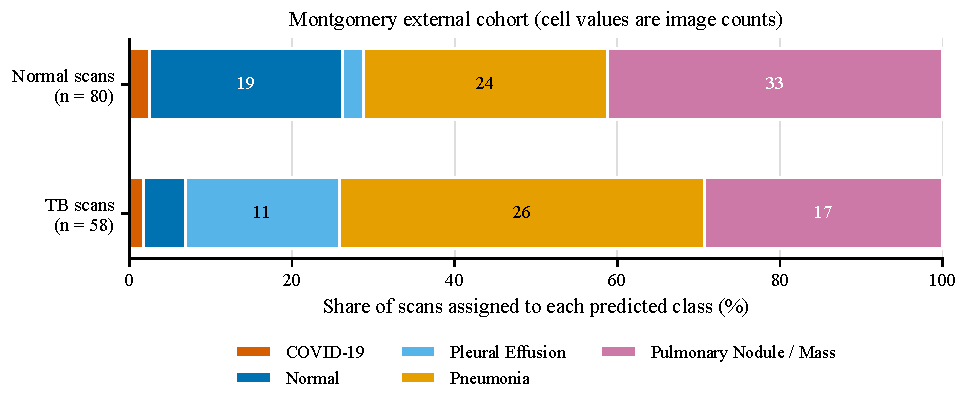
\includegraphics[width=\linewidth]{fig_external_breakdown.pdf}
\caption{Predicted class for the normal (left) and TB (right) radiographs of the external Montgomery cohort (selected model, scored once). The cohort contains no COVID-19, Pleural Effusion, Pneumonia or Nodule/Mass case.}
\label{fig:external}
\end{figure}

\subsection{Source-identifiability probe}
\label{sec:res-probe}
With ImageNet features the source was identified with balanced accuracy \RProbeImgBalAcc\% across \RProbeImgNSources{} sources (chance \RProbeImgChance\%; Table~\ref{tab:probe}), and it stayed identifiable within single classes: \RProbeImgWithinNormal\% among Normal images (chance \RProbeImgWithinNormalChance\%), \RProbeImgWithinTB\% among Tuberculosis, \RProbeImgWithinPneumonia\% among Pneumonia and \RProbeImgWithinCovid\% among COVID-19 images. Features of the trained backbone gave nearly identical values (\RProbeMdlBalAcc\% overall), as expected because fine-tuning changed only the last 17 weighted layers (verified by weight comparison). Source and class are confounded in this benchmark, and source information is linearly available in the features on which the classifier's head operates, so a source shortcut is possible. The probe does not show that the classifier uses it; we treat it as indirect evidence together with the per-source and external results.

\begin{table}[t]
\centering
\caption{Source-identifiability probe: balanced accuracy (\%) of a logistic regression predicting the source collection from frozen 1024-dimensional features on \RProbeNTest{} probe-test images (\RProbeNTrain{} probe-training images). ``Within'' rows use only images of that class. Chance is $1/S$ for $S$ sources.}
\label{tab:probe}
\small
\begin{tabular}{@{}lrrrr@{}}
\toprule
Images & Sources & Chance & ImageNet features & Trained backbone \\
\midrule
All classes & \RProbeImgNSources & \RProbeImgChance & \RProbeImgBalAcc & \RProbeMdlBalAcc \\
Within Normal & \RProbeImgWithinNormalNSources & \RProbeImgWithinNormalChance & \RProbeImgWithinNormal & \RProbeMdlWithinNormal \\
Within Tuberculosis & \RProbeImgWithinTBNSources & \RProbeImgWithinTBChance & \RProbeImgWithinTB & \RProbeMdlWithinTB \\
Within Pneumonia & \RProbeImgWithinPneumoniaNSources & \RProbeImgWithinPneumoniaChance & \RProbeImgWithinPneumonia & \RProbeMdlWithinPneumonia \\
Within COVID-19 & \RProbeImgWithinCovidNSources & \RProbeImgWithinCovidChance & \RProbeImgWithinCovid & \RProbeMdlWithinCovid \\
\bottomrule
\end{tabular}
\end{table}

\subsection{Seed variability and preprocessing ablation}
\label{sec:res-seeds}
Table~\ref{tab:seeds} reports the selected run and two further seeds (\RMSSeeds; \RMSNRuns{} runs on the same build, split and recipe). Internal results varied little: test accuracy had mean \RMSTestAccMean\% (SD \RMSTestAccSD, range \RMSTestAccMin--\RMSTestAccMax\%) and macro-F1 mean \RMSTestMacroFOneMean\% (SD \RMSTestMacroFOneSD, range \RMSTestMacroFOneMin--\RMSTestMacroFOneMax\%). The selected run is the highest of the three, within a spread of under one percentage point; a small favourable draw cannot be ruled out, and it was chosen before seeds \RMSRunTwoSeed{} and \RMSRunThreeSeed{} existed. External specificity varied more (mean \RMSExtSpecMean\%, range \RMSExtSpecMin--\RMSExtSpecMax\%), so differences of a few points in external specificity between runs of this recipe should not be interpreted. In every run, exact TB recall on Montgomery was \RMSExtTBMean\%, and specificity stayed low, so the external failure is consistent across seeds. The SD from three runs is a rough estimate and says nothing about other splits, data or architectures.

\begin{table}[t]
\centering
\caption{Seed variability of the selected configuration (build \RDatasetBuild). Test values in \%, except ROC-AUC; external specificity and exact TB recall in \%. Mean $\pm$ sample SD over three runs. The served model is run~2 regardless of these results.}
\label{tab:seeds}
\small
\begin{tabular}{@{}llrrrrr@{}}
\toprule
Run & Seed & Test acc. & Macro-F1 & Macro ROC-AUC & Ext. specificity & Ext. TB recall \\
\midrule
Run 2 (selected) & \RSeed & \RTestAcc & \RTestMacroFOne & \RTestMacroAUC & \RExtSpec & \RExtTB \\
Run 3 & \RMSRunTwoSeed & \RMSRunTwoTestAcc & \RMSRunTwoTestMacroFOne & \RMSRunTwoTestMacroAUC & \RMSRunTwoExtSpec & \RMSRunTwoExtTB \\
Run 4 & \RMSRunThreeSeed & \RMSRunThreeTestAcc & \RMSRunThreeTestMacroFOne & \RMSRunThreeTestMacroAUC & \RMSRunThreeExtSpec & \RMSRunThreeExtTB \\
\midrule
Mean $\pm$ SD & -- & \RMSTestAccMean{} $\pm$ \RMSTestAccSD & \RMSTestMacroFOneMean{} $\pm$ \RMSTestMacroFOneSD & \RMSTestMacroAUCMean{} $\pm$ \RMSTestMacroAUCSD & \RMSExtSpecMean{} $\pm$ \RMSExtSpecSD & \RMSExtTBMean{} $\pm$ \RMSExtTBSD \\
Min--max & -- & \RMSTestAccMin--\RMSTestAccMax & \RMSTestMacroFOneMin--\RMSTestMacroFOneMax & \RMSTestMacroAUCMin--\RMSTestMacroAUCMax & \RMSExtSpecMin--\RMSExtSpecMax & \RMSExtTBMin--\RMSExtTBMax \\
\bottomrule
\end{tabular}
\end{table}

In the preprocessing ablation (run~5, same seed, data and schedule, filters removed; Table~S6), test accuracy was \RAblTestAcc\% against \RMSRunOneTestAcc\% for the run with filters, macro-F1 \RAblTestMacroFOne\% against \RMSRunOneTestMacroFOne\% and macro ROC-AUC \RAblTestMacroAUC{} against \RMSRunOneTestMacroAUC. All three internal values lie below the whole seed range of runs 2--4, and the accuracy and macro-F1 differences are several times the seed SD, so in this single comparison the run with the filters scored higher internally by more than the seed-to-seed spread. External specificity was \RAblExtSpec\% against \RMSRunOneExtSpec\%, so removing the filters did not raise it. Run~5 named \RAblExtTB\% of the Montgomery TB scans Tuberculosis, a small number of scans, where no filtered run named any; this is an observation from one run. Run~5 also selected its last epoch (16 of 16, validation still rising), whereas runs 3 and 4 stopped early, so a difference in convergence speed cannot be excluded. With one ablation seed the difference cannot be separated from run-to-run variation outside the measured spread, and we make no claim about why the filters matter.

\subsection{C1: source and disease information by spatial-frequency band}
\label{sec:res-c1}
On the full cached image, ImageNet features gave source balanced accuracy \RSpecMainTestFullSrcBA\% (95\% interval \RSpecMainTestFullSrcBALo--\RSpecMainTestFullSrcBAHi\%; chance 16.7\%), within-source disease macro-F1 \RSpecMainTestFullFWs\%, six-class macro-F1 \RSpecMainTestFullFAll\% and within-Normal source accuracy \RSpecMainTestFullNormBA\% (test sample, $N=\RSpecMainTestN$; Table~\ref{tab:c1}, Fig.~\ref{fig:spectral}). The trained backbone and the no-filter cache gave source accuracy \RSpecServedTestFullSrcBA\% and \RSpecNofilterTestFullSrcBA\% and within-source macro-F1 \RSpecServedTestFullFWs\% and \RSpecNofilterTestFullFWs\% on the full image.

\textit{Source information is present in every band.} Band-pass source accuracy rose from \RSpecMainTestPassASrcBA\% in band A to \RSpecMainTestPassFSrcBA\% in band F, always above the 16.7\% chance level, with a dip at band B and a steep rise toward bands E and F. Within Normal images, source accuracy was \RSpecMainTestPassANormBA\% in band A and \RSpecMainTestPassFNormBA\% in band F, above the nominal 25\% in every band, so source information survives with disease held fixed. Disease information is also spread over the bands (within-source macro-F1 from \RSpecMainTestPassBFWs\% in band B to \RSpecMainTestPassFFWs\% in band F) and is highest in the high-frequency bands E and F, as is the source signal. Those bands may also be the ones most affected by resampling of different native grids and by the pre-filters.

\textit{No band is necessary.} Removing any single band left source accuracy nearly intact. The largest drop was \RSpecMainTestStopFDeltaS{} points for band F (interval \RSpecMainTestStopFDeltaSLo{} to \RSpecMainTestStopFDeltaSHi), the only band-stop whose interval excluded zero in that direction; removing band D shifted source accuracy the other way (\RSpecMainTestStopDDeltaS{} points, interval \RSpecMainTestStopDDeltaSLo{} to \RSpecMainTestStopDDeltaSHi). No band-stop reached the 5-point threshold fixed in advance, and all disease intervals included zero (the largest change was \RSpecMainTestStopEDeltaD{} points for band E). Source information is therefore redundant across bands in these features.

\textit{Sensitivity.} The profile of the trained backbone is close to the ImageNet profile (Fig.~\ref{fig:spectral}a). The no-filter cache shows the same shape, with a dip at band B and a rise toward E and F, but its levels differ: source accuracy is lower in the high bands (band E \RSpecNofilterTestPassESrcBA\% against \RSpecMainTestPassESrcBA\%, band F \RSpecNofilterTestPassFSrcBA\% against \RSpecMainTestPassFSrcBA\%, with non-overlapping intervals for band E) and slightly higher in bands A to C. This is consistent with the pre-filters and resampling contributing to the high-band source signal; it is a sensitivity result, not a test, and the per-band values of both checks are in Table~S7. The null result holds in all three: no band stands out as the carrier. Availability in frozen features does not show that the trained model uses the information.

\begin{table}[t]
\centering
\caption{C1 on the test sample (ImageNet features, primary; $N=\RSpecMainTestN$ images, \RSpecMainTestNWithinSources{} sources in the within-source score). Band-pass: source balanced accuracy with 95\% bootstrap interval over scored images, within-source disease macro-F1 and within-Normal source accuracy (\%). Band-stop: $dS$ and $dD$ are the full-image value minus the band-stop value in percentage points, with 95\% intervals. Chance for source accuracy is 16.7\%. One probe fit per variant; intervals cover test-sample variation only.}
\label{tab:c1}
\footnotesize
\setlength{\tabcolsep}{3pt}
\begin{tabular}{@{}lcrrcc@{}}
\toprule
 & \multicolumn{3}{c}{Band-pass} & \multicolumn{2}{c}{Band-stop} \\
\cmidrule(lr){2-4}\cmidrule(lr){5-6}
Band & Source acc. (95\% int.) & Within-source F1 & Within-Normal src. & $dS$ (95\% int.) & $dD$ (95\% int.) \\
\midrule
A & \RSpecMainTestPassASrcBA{} (\RSpecMainTestPassASrcBALo--\RSpecMainTestPassASrcBAHi) & \RSpecMainTestPassAFWs & \RSpecMainTestPassANormBA & \RSpecMainTestStopADeltaS{} (\RSpecMainTestStopADeltaSLo{} to \RSpecMainTestStopADeltaSHi) & \RSpecMainTestStopADeltaD{} (\RSpecMainTestStopADeltaDLo{} to \RSpecMainTestStopADeltaDHi) \\
B & \RSpecMainTestPassBSrcBA{} (\RSpecMainTestPassBSrcBALo--\RSpecMainTestPassBSrcBAHi) & \RSpecMainTestPassBFWs & \RSpecMainTestPassBNormBA & \RSpecMainTestStopBDeltaS{} (\RSpecMainTestStopBDeltaSLo{} to \RSpecMainTestStopBDeltaSHi) & \RSpecMainTestStopBDeltaD{} (\RSpecMainTestStopBDeltaDLo{} to \RSpecMainTestStopBDeltaDHi) \\
C & \RSpecMainTestPassCSrcBA{} (\RSpecMainTestPassCSrcBALo--\RSpecMainTestPassCSrcBAHi) & \RSpecMainTestPassCFWs & \RSpecMainTestPassCNormBA & \RSpecMainTestStopCDeltaS{} (\RSpecMainTestStopCDeltaSLo{} to \RSpecMainTestStopCDeltaSHi) & \RSpecMainTestStopCDeltaD{} (\RSpecMainTestStopCDeltaDLo{} to \RSpecMainTestStopCDeltaDHi) \\
D & \RSpecMainTestPassDSrcBA{} (\RSpecMainTestPassDSrcBALo--\RSpecMainTestPassDSrcBAHi) & \RSpecMainTestPassDFWs & \RSpecMainTestPassDNormBA & \RSpecMainTestStopDDeltaS{} (\RSpecMainTestStopDDeltaSLo{} to \RSpecMainTestStopDDeltaSHi) & \RSpecMainTestStopDDeltaD{} (\RSpecMainTestStopDDeltaDLo{} to \RSpecMainTestStopDDeltaDHi) \\
E & \RSpecMainTestPassESrcBA{} (\RSpecMainTestPassESrcBALo--\RSpecMainTestPassESrcBAHi) & \RSpecMainTestPassEFWs & \RSpecMainTestPassENormBA & \RSpecMainTestStopEDeltaS{} (\RSpecMainTestStopEDeltaSLo{} to \RSpecMainTestStopEDeltaSHi) & \RSpecMainTestStopEDeltaD{} (\RSpecMainTestStopEDeltaDLo{} to \RSpecMainTestStopEDeltaDHi) \\
F & \RSpecMainTestPassFSrcBA{} (\RSpecMainTestPassFSrcBALo--\RSpecMainTestPassFSrcBAHi) & \RSpecMainTestPassFFWs & \RSpecMainTestPassFNormBA & \RSpecMainTestStopFDeltaS{} (\RSpecMainTestStopFDeltaSLo{} to \RSpecMainTestStopFDeltaSHi) & \RSpecMainTestStopFDeltaD{} (\RSpecMainTestStopFDeltaDLo{} to \RSpecMainTestStopFDeltaDHi) \\
\midrule
Full image & \RSpecMainTestFullSrcBA{} (\RSpecMainTestFullSrcBALo--\RSpecMainTestFullSrcBAHi) & \RSpecMainTestFullFWs & \RSpecMainTestFullNormBA & -- & -- \\
\bottomrule
\end{tabular}
\end{table}

\begin{figure}[t]
\centering
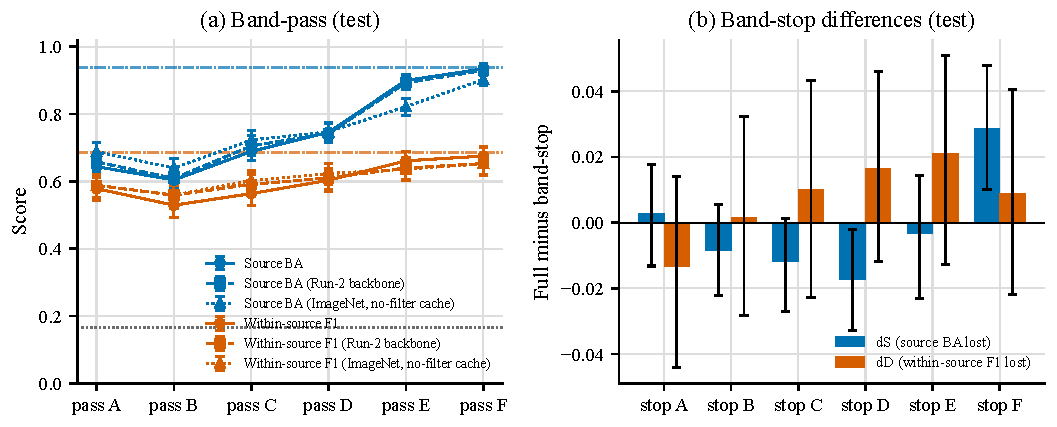
\includegraphics[width=\linewidth]{fig_spectral_map.pdf}
\caption{C1 on the test sample. (a) Band-pass variants A--F: source balanced accuracy (blue) and within-source disease macro-F1 (orange), both on the same score axis. Solid lines: ImageNet features (primary); dashed: run-2 backbone (secondary; it saw all six sources in training); dotted: ImageNet features of the no-filter cache (sensitivity check). The dotted grey horizontal line is the 16.7\% chance level for source accuracy; the dash-dot horizontal lines are the full-image levels of the primary extractor. (b) Band-stop differences, full image minus band-stop image, for source accuracy ($dS$) and within-source macro-F1 ($dD$). Error bars are 95\% bootstrap intervals over the scored images (one probe fit per variant; training variance is not included).}
\label{fig:spectral}
\end{figure}

\subsection{C3: linear erasure of source information}
\label{sec:res-c3}
Both extractors reached the cap of \RInlpImgKStar{} iterations ($k^\ast=\RInlpImgKStar$, stopped by the \RInlpImgStoppedBy), not the stopping threshold (Table~\ref{tab:inlp}, Fig.~\ref{fig:inlp}). With ImageNet features, the source balanced accuracy a fresh linear probe could reach fell from \RInlpImgTestSrcBAKZero\% at $k=0$ to \RInlpImgTestSrcBAKStar\% at $k^\ast$ on the test split ($N=\RInlpImgNTest$): a large reduction, but not to chance, so the source information was not removed by this linear route within the cap. Disease scores fell as well. The within-source macro-F1 changed by \RInlpImgTestChangeFWsKStar{} points (95\% interval \RInlpImgTestChangeFWsKStarLo{} to \RInlpImgTestChangeFWsKStarHi), the six-class macro-F1 by \RInlpImgTestChangeFAllKStar{} points (\RInlpImgTestChangeFAllKStarLo{} to \RInlpImgTestChangeFAllKStarHi), accuracy from \RInlpImgTestAccKZero\% to \RInlpImgTestAccKStar\% and macro ROC-AUC from \RInlpImgTestAUCKZero{} to \RInlpImgTestAUCKStar. Both intervals exclude zero, which is consistent with source and disease information being entangled in these features. The six-class drop exceeds the within-source drop, which is consistent with part of the six-class score being bought with source cues.

Removing all linearly decodable source information in a single step with LEACE (source accuracy at chance in the fit) lowered the six-class macro-F1 by \RInlpImgTestChangeFAllLeace{} points (compare the INLP loss at 20 iterations in the previous paragraph), and the within-source score by \RInlpImgTestChangeFWsLeace{} points. The trained backbone behaved similarly: source accuracy fell from \RInlpMdlTestSrcBAKZero\% to \RInlpMdlTestSrcBAKStar\% and the within-source macro-F1 changed by \RInlpMdlTestChangeFWsKStar{} points (\RInlpMdlTestChangeFWsKStarLo{} to \RInlpMdlTestChangeFWsKStarHi); these numbers come from a backbone that saw all sources and are not held-out results.

On Montgomery (Normal and Tuberculosis only, scored once; not untouched), ImageNet-feature heads had sensitivity \RInlpImgExtSensKZero\% (\RInlpImgExtSensKZeroK/\RInlpImgExtSensKZeroN) and specificity \RInlpImgExtSpecKZero\% (\RInlpImgExtSpecKZeroK/\RInlpImgExtSpecKZeroN) at $k=0$, and sensitivity \RInlpImgExtSensKStar\% and specificity \RInlpImgExtSpecKStar\% (Wilson interval \RInlpImgExtSpecKStarLo--\RInlpImgExtSpecKStarHi\%) at $k^\ast$. The specificity intervals overlap, the scans are the same at both settings so the intervals are not independent, and the cohort has 138 images; no conclusion about a change in specificity is drawn.

\begin{table}[t]
\centering
\caption{C3 on the full test split (ImageNet features, primary; $N=\RInlpImgNTest$). A fresh linear probe measures the source accuracy after projection; the disease head is retrained on the projected features. Percentages except ROC-AUC. LEACE: closed form, source accuracy at chance in the fit.}
\label{tab:inlp}
\small
\begin{tabular}{@{}lrrrrr@{}}
\toprule
Setting & Source acc. & Within-source F1 & Six-class macro-F1 & Accuracy & Macro ROC-AUC \\
\midrule
$k=0$ (no erasure) & \RInlpImgTestSrcBAKZero & \RInlpImgTestFWsKZero & \RInlpImgTestFAllKZero & \RInlpImgTestAccKZero & \RInlpImgTestAUCKZero \\
INLP, $k^\ast=\RInlpImgKStar$ & \RInlpImgTestSrcBAKStar & \RInlpImgTestFWsKStar & \RInlpImgTestFAllKStar & \RInlpImgTestAccKStar & \RInlpImgTestAUCKStar \\
LEACE & \RInlpImgLeaceTestSrcBA & \RInlpImgLeaceTestFWs & \RInlpImgLeaceTestFAll & \RInlpImgLeaceTestAcc & \RInlpImgLeaceTestAUC \\
\bottomrule
\end{tabular}
\end{table}

\begin{figure}[t]
\centering
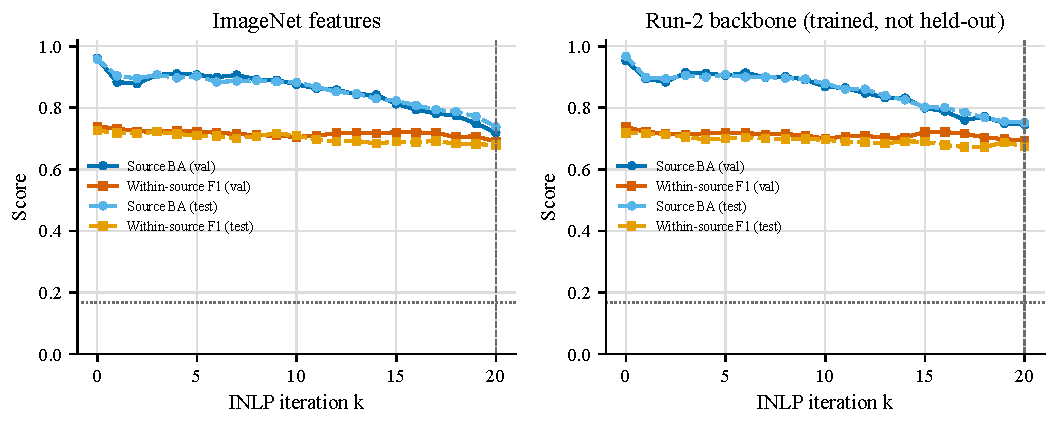
\includegraphics[width=\linewidth]{fig_inlp.pdf}
\caption{C3: source balanced accuracy of a fresh linear probe (blue) and within-source disease macro-F1 of the retrained head (orange) against INLP iteration $k$, on validation (solid) and test (dashed). Left: ImageNet features (primary). Right: run-2 backbone (secondary; trained on all six sources, so not held-out). The values at $k=0$ are the full-image levels without erasure. The dotted grey line is the 16.7\% chance level for source accuracy; the vertical dashed line marks the iteration cap of 20. Intervals are not drawn here; bootstrap 95\% intervals over test images for the changes at $k^\ast$ are given in the text.}
\label{fig:inlp}
\end{figure}

\subsection{C4: linear-head leave-one-source-out}
\label{sec:res-c4}
For \RLosoImgNIncluded{} sources, Table~\ref{tab:loso} and Fig.~\ref{fig:loso} give the macro-F1 of a linear head trained on the other five sources, on the evaluated classes of the held-out source, with the in-distribution reference and the gap (reference minus held-out). On four of the five sources the held-out score was far below the reference: the gap was \RLosoImgCohenGap{} points for the COVID-19 image data collection, \RLosoImgKermanyGap{} for Kermany, \RLosoImgShenzhenGap{} for Shenzhen and \RLosoImgTBXkGap{} for TBX11K, the largest. The trained-backbone matrix is similar (macro-F1 \RLosoMdlCohenMacroFOne\%, \RLosoMdlKermanyMacroFOne\%, \RLosoMdlShenzhenMacroFOne\% and \RLosoMdlTBXkMacroFOne\% for the same four sources) but is not a held-out test.

The NIH gap is negative (\RLosoImgNIHGap{} points, interval \RLosoImgNIHGapLo{} to \RLosoImgNIHGapHi; trained backbone \RLosoMdlNIHGap, interval \RLosoMdlNIHGapLo{} to \RLosoMdlNIHGapHi), but this is a metric artefact and should not be read as better generalisation. NIH has only two testable classes, and the six-class reference head also predicts the NIH-only classes Effusion and Nodule/Mass, which count as errors for the two evaluated classes; the reference is therefore low (\RLosoImgNIHRefMacroFOne\% with ImageNet features). Likewise, balanced accuracy below 50\% for a two-class source (TBX11K \RLosoImgTBXkBalAcc\%, COVID-19 image data collection \RLosoImgCohenBalAcc\%) reflects predictions of non-evaluated classes counted as errors, not a head worse than chance on a binary question. A chance-referenced reading comes from the binary abnormal-versus-normal view, in which the ROC-AUC of $1-P(\text{Normal})$ was \RLosoImgKermanyBinAUC{} for Kermany, \RLosoImgNIHBinAUC{} for NIH, \RLosoImgShenzhenBinAUC{} for Shenzhen and \RLosoImgTBXkBinAUC{} for TBX11K; the two TB sources, Shenzhen and TBX11K, are the lowest. This is consistent with dependence on source-specific cues and with class--source confounding, but it does not identify which cues. The COVID-19 image data collection has only \RLosoImgCohenN{} test images in its evaluated classes and its result is very uncertain.

Scored once with the head trained on all six sources, Montgomery gave sensitivity \RLosoImgExtSens\% and specificity \RLosoImgExtSpec\% with ImageNet features, and \RLosoMdlExtSens\% and \RLosoMdlExtSpec\% with the trained backbone (not untouched; 138 images). Every held-out number carries the patient-identity caveat of Section~\ref{sec:split}: TBX11K and COVID-19 Radiography rows are grouped per image and Kermany identities are derived from file names, so patient separation within those sources is not proven, and the reference scores in particular may be optimistic for them.

\begin{table}[t]
\centering
\caption{C4: macro-F1 (\%) on the evaluated classes of the held-out source for a linear head trained on the other five sources (ImageNet features, primary), with 95\% bootstrap interval over held-out test images, the in-distribution reference (head trained on all six sources, same images), the gap (reference minus held-out, in points) and the binary abnormal-versus-normal ROC-AUC where defined. Predictions of non-evaluated classes count as errors. $N$ is the number of test images in the evaluated classes.}
\label{tab:loso}
\small
\begin{tabular}{@{}lrcrrr@{}}
\toprule
Held-out source & $N$ & Held-out macro-F1 (95\% int.) & Reference & Gap & Binary AUC \\
\midrule
COVID-19 image data collection & \RLosoImgCohenN & \RLosoImgCohenMacroFOne{} (\RLosoImgCohenMacroFOneLo--\RLosoImgCohenMacroFOneHi) & \RLosoImgCohenRefMacroFOne & \RLosoImgCohenGap & -- \\
Kermany & \RLosoImgKermanyN & \RLosoImgKermanyMacroFOne{} (\RLosoImgKermanyMacroFOneLo--\RLosoImgKermanyMacroFOneHi) & \RLosoImgKermanyRefMacroFOne & \RLosoImgKermanyGap & \RLosoImgKermanyBinAUC \\
NIH ChestX-ray14 & \RLosoImgNIHN & \RLosoImgNIHMacroFOne{} (\RLosoImgNIHMacroFOneLo--\RLosoImgNIHMacroFOneHi) & \RLosoImgNIHRefMacroFOne & \RLosoImgNIHGap & \RLosoImgNIHBinAUC \\
Shenzhen & \RLosoImgShenzhenN & \RLosoImgShenzhenMacroFOne{} (\RLosoImgShenzhenMacroFOneLo--\RLosoImgShenzhenMacroFOneHi) & \RLosoImgShenzhenRefMacroFOne & \RLosoImgShenzhenGap & \RLosoImgShenzhenBinAUC \\
TBX11K & \RLosoImgTBXkN & \RLosoImgTBXkMacroFOne{} (\RLosoImgTBXkMacroFOneLo--\RLosoImgTBXkMacroFOneHi) & \RLosoImgTBXkRefMacroFOne & \RLosoImgTBXkGap & \RLosoImgTBXkBinAUC \\
\bottomrule
\end{tabular}
\end{table}

\begin{figure}[t]
\centering
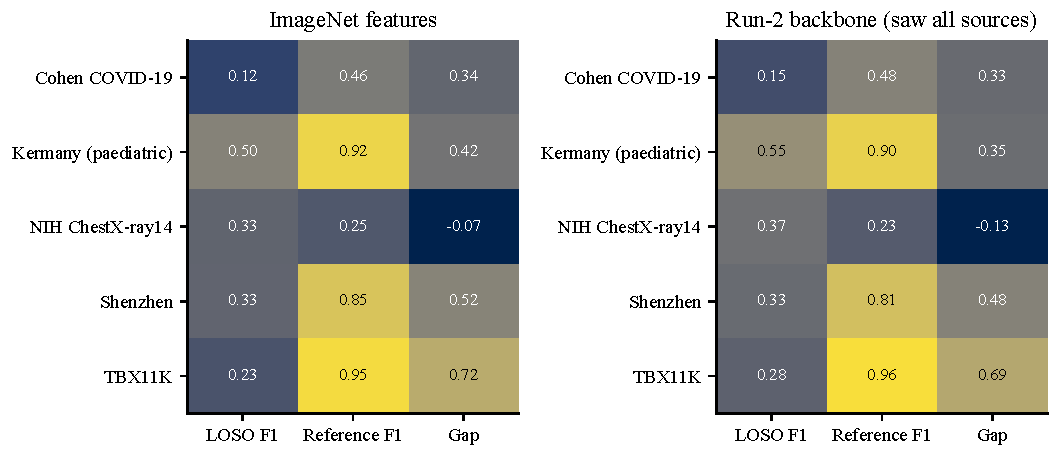
\includegraphics[width=\linewidth]{fig_loso_matrix.pdf}
\caption{C4: macro-F1 on the evaluated classes of the held-out source (``LOSO F1''; predictions of other classes count as errors), the in-distribution reference F1 and the gap (reference minus held-out), as fractions from 0 to 1 on one colour scale. Left: ImageNet features (primary). Right: run-2 backbone (secondary; it saw all six sources, so this is not a held-out or external test). Intervals are not drawn in the figure; 95\% bootstrap intervals over held-out test images are in Table~\ref{tab:loso}. The negative NIH gap is a metric artefact explained in the text. Patient-identity caveat: separation is proven only for rows with known identity.}
\label{fig:loso}
\end{figure}

\subsection{C2: decision not to retrain}
\label{sec:res-c2}
The go/no-go rule fixed in advance returned \RBsDecision. Criterion~1 \RBsConditionOne{} (\RBsNBandsSatisfying{} bands satisfied it; the band with the largest source drop was band \RBsBand), so the matched-energy random control was not run (criterion~2 \RBsConditionTwo), criterion~3 \RBsConditionThree{} and criterion~4 (the student's approval of compute) was moot. In the selection step for band \RBsBand{} the validation source-accuracy drop was \RSpecMainValStopFDeltaS{} points, below the 5-point threshold, and the upper bound of the disease change (\RSpecMainValStopFDeltaDHi{} points) also exceeded the 3-point limit. In the exploratory C2-lite step (ImageNet features, band \RBsBand{} removed, \RBsLiteValNTrain{} training images), the validation source-accuracy drop was \RBsLiteValDeltaS{} points (95\% interval \RBsLiteValDeltaSLo{} to \RBsLiteValDeltaSHi) and the disease change \RBsLiteValDeltaD{} points (\RBsLiteValDeltaDLo{} to \RBsLiteValDeltaDHi); on the test table, scored once and labelled exploratory, the values were \RBsLiteTestDeltaS{} points (\RBsLiteTestDeltaSLo{} to \RBsLiteTestDeltaSHi) and \RBsLiteTestDeltaD{} points (\RBsLiteTestDeltaDLo{} to \RBsLiteTestDeltaDHi). Removing the best single band thus lowered the source accuracy of a linear head by a few points, and the disease change was not distinguishable from zero. We report this as a negative result of the band-stop idea within this protocol and frozen features. No band-stop network was trained, so there is no C2 number and no statement about suppression in a trained network; C2 is future work.

\section{Discussion}
\label{sec:discussion}

\subsection{What the measurements show}
With patient- and duplicate-grouped splits and no proxy labels, a standard DenseNet-121 reached an internal test accuracy of \RTestAcc\% and a macro ROC-AUC of \RTestMacroAUC. On radiographs from a hospital it had never seen, it flagged \RExtSensK/\RExtSensN{} TB scans as abnormal but called only \RExtSpecK/\RExtSpecN{} normal scans Normal, and named \RExtTBK/\RExtTBN{} TB scans Tuberculosis. The internal results therefore overstate behaviour at an unseen hospital by a wide margin, although the usual leakage paths were closed for sources with patient identifiers. Closing the leakage paths made the internal estimate credible but left it a poor guide to generalisation.

The new analyses address one possible reason, source confounding. Source information is available throughout the spectrum: the source of an image can be recovered from every one of six octave bands, including within Normal images, and removing a single band changes little (Section~\ref{sec:res-c1}). The information is also entangled with disease information: twenty steps of linear erasure lowered the source accuracy a fresh probe could reach from \RInlpImgTestSrcBAKZero\% to \RInlpImgTestSrcBAKStar\%, not to chance, and cost disease performance, and erasing the linearly decodable information in one step cost more (Section~\ref{sec:res-c3}). Finally, a linear head trained without a source scored far below its in-distribution reference on four of five held-out sources (Section~\ref{sec:res-c4}). These are measurements on frozen features. Together with the per-source and external results they are consistent with a model that depends on source-specific cues, but each is indirect: a probe shows that information is available, not that the trained network uses it, and we make no causal claim about the shortcut or about its location. For the same reason we do not write that source information ``cannot be removed'': only linear erasure, a 20-iteration cap, one cache, one benchmark and one run were examined, and a probe near chance would not prove absence either.

\paragraph{Novelty and its limits} To our knowledge, within the searches described, no prior work quantifies, band by band, source versus disease information in CNN features of chest radiographs. That statement concerns only the localisation in C1, and its main outcome is that the signal is not localised. Per-band harmonisation~\cite{kim2023homogenization} and spectral failure analysis~\cite{halimi2026spectral} exist for chest radiographs, so we do not claim frequency-filtered source classification as new in general. Linear erasure~\cite{ravfogel2020null,belrose2023leace} and leave-one-source-out evaluation~\cite{yao2019strong} are published; here they are measurements, and neither is claimed as a method or a protocol contribution. The negative C2 decision is part of the contribution: the rule, fixed in advance, prevented a retraining that the frozen-feature evidence did not support, and we make no claim about band suppression in a trained network.

\paragraph{Caveats that bound these readings}
(i)~The cache is resampled to $224\times224$ after filtering, and sources differ in native resolution and field of view; the high bands in particular may reflect resampling and the pre-filters, and the lower high-band source accuracy of the no-filter cache is consistent with that. No claim about scanner physics is made. (ii)~The secondary extractor was trained on all six sources, so trained-backbone numbers are not held-out. (iii)~Disease and source are confounded (Effusion and Nodule/Mass occur only in NIH), which is why the within-source disease score is primary. (iv)~Intervals cover test-sample variation only, with one probe fit per variant; samples are small (150 and 100 images per cell) and only five sources have two classes with at least 20 images. (v)~The NIH gap in C4 is a metric artefact (Section~\ref{sec:res-c4}). (vi)~Patient identity is unknown for TBX11K and COVID-19 Radiography rows and derived from file names for Kermany, so every held-out number carries that caveat. (vii)~Montgomery is not untouched: it was scored for runs 1--5 and in C3 and C4, and run~2 was started after run~1's external results were seen. (viii)~Everything is one run per analysis with no seeds.

\subsection{Ranking versus operating point}
The external ROC-AUC of the abnormality score (\RExtAUC) is well above chance while specificity is low, just as internal macro ROC-AUC is much higher than internal accuracy. A shift of scores toward ``abnormal'' at a new hospital can leave the ranking partly intact and still move most normal images across the arg-max boundary. A model deployed at a new site would need its operating point re-established there. We do not compare these numbers with those of other studies, which used different data and splits.

\subsection{What the audit of the earlier pipeline showed}
\label{sec:disc-audit}
The V5 pipeline pooled eight public sources, several from third-party redistributions, and recorded an internal test accuracy of \RVFiveAcc\% on $N=\RVFiveN$ images. A retrospective audit found that 154 of the 1,570 internal test images (9.8\%) belonged to patients who also had images in the training split, and that 8,478 further images had no real patient identity, so their separation could not be checked. About half of the Pneumonia class (1,395 labels) consisted of TBX11K images labelled ``sick but non-TB'', 124 Tuberculosis labels were latent TB, and 1,440 of 1,467 VinDr-CXR images used as single-label examples carried two or more findings. On Montgomery every recorded V5 variant flagged essentially every TB radiograph as abnormal but called none of the normal radiographs Normal (specificity \RVFiveExtSpecK/\RVFiveExtSpecN); a sensitivity quoted alone would have suggested a perfect screening tool. One V5 TB source is described as containing Montgomery images, and a content check could neither confirm nor exclude the overlap. Earlier drafts also contained reporting errors, and the canonical checkpoint was lost. V6 removes each defect or measures it explicitly. The V5 numbers are not comparable with V6.

\subsection{Implications for multi-source benchmark design}
The audit and the analyses suggest the following practices: acquire from official sources and log provenance per file; fix labelling rules before training and label only from the source's own labels; split by patient and by content, stating how many images have unknown identity; report results per source and flag classes supplied by one source; evaluate on an unseen hospital and always report specificity with sensitivity; and fix selection rules in advance (here recorded in the repository, not registered externally). Because source information is linearly available throughout the spectrum, these results give no reason to expect that band filtering or linear erasure of frozen features would make up for source confounding; source-balanced data were not tested.

\subsection{Input gate}
\label{sec:disc-gate}
The application refuses images judged not to be chest radiographs, using a heuristic score because the intended trained gate was unavailable. At the inherited threshold (0.83) it rejected \RCxrGateBOneOldTestRej{} of \RCxrGateBOneOldTestN{} genuine radiographs of the build-1 test split (\RCxrGateBOneOldTestRejPct\%). After recalibration on build-2 validation radiographs only (threshold \RCxrGateNewThr), it rejected \RCxrGateBTwoNewTestRej{} of \RCxrGateBTwoOldTestN{} build-2 test radiographs (\RCxrGateBTwoNewTestRejPct\%), against \RCxrGateBTwoOldTestRej{} (\RCxrGateBTwoOldTestRejPct\%) at 0.83 on the same split. The negatives used for calibration are synthetic and few, so the gate's ability to reject real non-radiographs is not established.
\subsection{Limitations}
\label{sec:limitations}
\begin{itemize}
\item \textbf{Frozen features, linear methods, one benchmark.} C1, C3 and C4 examine linear probes and heads on frozen DenseNet-121 features of one cache, with six sources and one run each. They say nothing about fine-tuned networks, nonlinear erasure or other data. No retraining per held-out source was done, so the served model is not shown to behave as the C4 heads do.
\item \textbf{Few training runs, CPU, time-boxed.} Run~1 is a single run, run~2 has two further seeds, and the ablation has one seed; the SD of test accuracy (\RMSTestAccSD{} points) is a rough estimate that does not extend to other splits, data or architectures.
\item \textbf{Limited ablation.} Only the full chain and no filtering were compared; single filters, the order relative to resizing and alternative backbones were not studied. Run~5 selected its last epoch.
\item \textbf{One small, binary external cohort}, not strictly untouched.
\item \textbf{Label quality and the single-label assumption.} NIH labels are mined from reports; images with several findings were excluded.
\item \textbf{Population and source confounding.} Kermany images are paediatric, all others adult; no demographic data were available, so subgroup performance~\cite{seyyedkalantari2021underdiagnosis} could not be assessed.
\item \textbf{Uncalibrated scores and unvalidated thresholds.} No calibration map was fitted, and the application's 0.5 ``inconclusive'' threshold is not validated.
\item \textbf{No clinical validation.} The system has not been evaluated prospectively or by radiologists and must not be used for diagnosis.
\end{itemize}

\subsection{Future work}
In order: a causal test of the source shortcut in a trained network (leave-one-source-out training and lung-masked inference); the C2 band-stop retraining only if new evidence justifies it, under a rule again fixed in advance; a phase-versus-amplitude split per band; nonlinear erasure; more seeds, so that runs can be compared as distributions; a second backbone; access to VinDr-CXR and JSRT so that Effusion and Nodule/Mass have more than one source; a second external cohort with more classes, ideally a local set collected with ethics approval; and evaluation of the input gate on real non-radiographs.

\section{Conclusion}
\label{sec:conclusion}

We rebuilt a multi-source six-class chest radiograph benchmark from official sources with labelling rules fixed before training, patient- and duplicate-grouped splits (separation proven only where patient identity is known) and a held-out external cohort, and used it to examine source shortcuts in a standard DenseNet-121. Internal test accuracy was \RTestAcc\% (Wilson 95\% interval \RTestAccLo--\RTestAccHi\%), yet only \RExtSpecK{} of \RExtSpecN{} normal external radiographs were called Normal and \RExtTBK{} of \RExtTBN{} TB radiographs were named Tuberculosis, consistently across three seeds.

In frozen features, source information was recoverable from every spatial-frequency band, from \RSpecMainTestPassASrcBA\% to \RSpecMainTestPassFSrcBA\% balanced accuracy against a chance level of 16.7\%, and no single band was necessary for it. To our knowledge, within the searches described, this band-by-band localisation of source versus disease information has not been reported for chest radiographs; its outcome is that the signal is not localised. Linear erasure lowered the recoverable source information from \RInlpImgTestSrcBAKZero\% to \RInlpImgTestSrcBAKStar\%, not to chance, and lowered disease scores too, consistent with entanglement. A linear head trained without one source scored \RLosoImgCohenGap{} to \RLosoImgTBXkGap{} points below its in-distribution reference on four of five held-out sources. The planned band-stop retraining was not run because the rule fixed in advance returned \RBsDecision, an outcome we record as part of the design. These results come from linear methods on frozen features of one benchmark and one run, carry the patient-identity caveat, and are indirect evidence about what a trained model uses.

For multi-source chest radiograph work the practical lesson is modest: document provenance, fix label rules in advance, group splits by patient and content, report per source, evaluate on an unseen hospital with sensitivity and specificity together, and note that these results give no reason to expect frequency filtering or linear erasure of frozen features to replace source-balanced data, which we did not test. We make no claim of clinical validity.


%% Declarations for the IMU submission. Included at the end of main.tex and
%% also to be pasted into the submission system where Elsevier asks for them.
%% Everything marked [AUTHORS TO CONFIRM] or [STUDENT TO CONFIRM] must be
%% checked and edited by the authors. Nothing here has been signed or approved.

\section*{CRediT authorship contribution statement}
\confirm{[AUTHORS TO CONFIRM] roles below are a proposal based on the project record; each author must confirm or edit their own roles, and all authors must approve the manuscript before submission. The author order is confirmed by the project owner; the corresponding author is [TO BE CONFIRMED]}

\textbf{Katkam Sathwik:} Conceptualization, Methodology, Software, Data curation, Formal analysis, Investigation, Validation, Visualization, Writing -- original draft, Writing -- review \& editing.
\textbf{Nagavelli Ramana:} Supervision, Conceptualization, Project administration, Writing -- review \& editing.
\textbf{P. Tirupathi:} Methodology, Writing -- review \& editing.
\textbf{K. Srinivas:} Methodology, Writing -- review \& editing.

\section*{Declaration of competing interest}
The authors declare that they have no known competing financial interests or personal relationships that could have appeared to influence the work reported in this paper. \confirm{each author confirms}

\section*{Funding}
This research did not receive any specific grant from funding agencies in the public, commercial, or not-for-profit sectors. \confirm{no funding}

\section*{Ethics statement}
\student{draft wording; please confirm with the institution}
No ethics approval was required for this study. It used only publicly available, de-identified chest radiograph collections that their publishers released for research use (listed under Data availability). No new images were acquired, no patients or other participants were recruited or contacted, no identifiable private information was accessed, and no attempt was made to re-identify any individual. The work is a secondary analysis of existing public data and therefore does not constitute research with human participants that requires informed consent. \confirm{whether the institution requires a formal ethics exemption or waiver for secondary analysis of public de-identified data; if one was obtained, give the committee name and reference number here; otherwise state that none was sought}

\section*{Data availability}
The images cannot be redistributed under the terms of several sources, and are not included in any repository. All sources are publicly available from their publishers:
\begin{itemize}
\item NIH ChestX-ray14: \url{https://nihcc.app.box.com/v/ChestXray-NIHCC}
\item Kermany et al., Mendeley Data v2 (DOI 10.17632/rscbjbr9sj.2): \url{https://data.mendeley.com/datasets/rscbjbr9sj/2}
\item Shenzhen Hospital CXR set (NLM): \url{https://data.lhncbc.nlm.nih.gov/public/Tuberculosis-Chest-X-ray-Datasets/Shenzhen-Hospital-CXR-Set/index.html}
\item Montgomery County CXR set (NLM): \url{https://data.lhncbc.nlm.nih.gov/public/Tuberculosis-Chest-X-ray-Datasets/Montgomery-County-CXR-Set/MontgomerySet/index.html}
\item COVID-19 image data collection (Git commit \texttt{78543292f8b0}): \url{https://github.com/ieee8023/covid-chestxray-dataset}
\item TBX11K: \url{https://mmcheng.net/tb/}
\item COVID-19 Radiography Database: \url{https://www.kaggle.com/datasets/tawsifurrahman/covid19-radiography-database}
\end{itemize}
The labelling rules, the dataset builder, the per-file provenance logs (URL, size, SHA-256), the build reports with split fingerprints and the manifests listing every image identifier and its split are available with the code, so that the identical partition can be rebuilt from the official sources. The protocol of the source-information analyses, its change log and the access log, and the result files of the spectral map, the erasure analysis, the leave-one-source-out analysis and the C2 decision are also kept in the repository.

\section*{Code availability}
The source code for acquisition, dataset construction, training, evaluation, the source-information analyses and the application, together with the configuration files and evaluation reports, will be made available at \confirm{repository URL; public release on acceptance or at submission} under \confirm{licence}. The trained checkpoint is identified by its SHA-256 digest in the configuration and can be shared on request \confirm{availability of model weights}.

\section*{Declaration of generative AI and AI-assisted technologies in the writing process}
\confirm{[AUTHORS TO CONFIRM] this statement is a draft; the authors must review and edit it so that it accurately describes how AI tools were used}

During the preparation of this work the authors used Claude (Anthropic), an AI assistant operated through the Claude Code environment, to draft and edit sections of the manuscript text and documentation from the project's records, and to assist with writing and reviewing parts of the analysis and evaluation code, including the code for dataset construction, training, the source-information analyses and the generation of result tables. The work was carried out under the supervision of the authors, who specified the study design and the decision rules, ran or checked the analyses, and verified the results. All numerical results in the manuscript are produced by the project's code from saved model outputs and inserted automatically, not written by the AI tool. After using this tool, the authors reviewed and edited the content as needed and take full responsibility for the content of the publication.


\bibliographystyle{elsarticle-num}
\bibliography{../shared/references}

\end{document}
